\section{Steuerungsplatinen}
\subsection{Motorregleransteuerung}
\subsubsection{Aufgaben \& verwendete Bauteile}
Diese wandeln die entsprechenden vom CAN-Bus übertragenen Daten mithilfe ihres 16-bit Timers (Timer1 des ATMEGA328p) in ein für unseren Motorregler verständliches PWM-Muster um.
Gleichzeitig übermitteln sie die von den Motorreglern übertragenen Telemetriedaten an den Controller des Lenkers.

\begin{minipage}{8.5cm}
    \begin{tikzpicture}
        \node[anchor=south west,inner sep=0] (image) at (0,0) {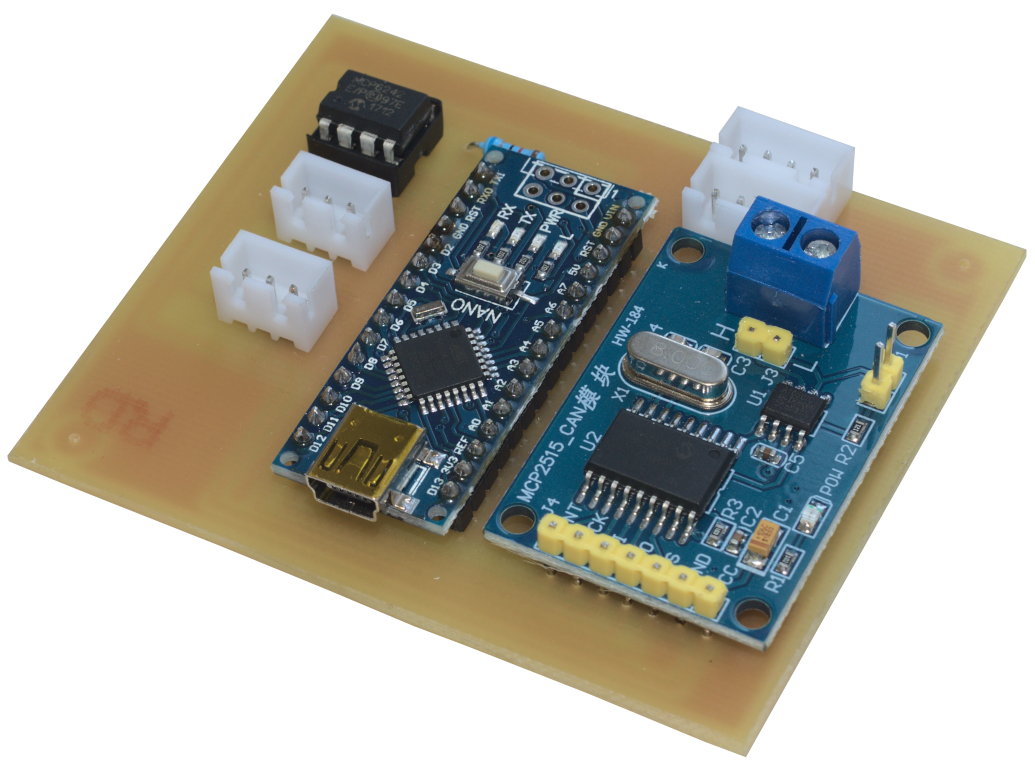
\includegraphics[width=0.9\textwidth]{Fotos/Regler_Platine.png}};
        \begin{scope}[x={(image.south east)},y={(image.north west)}]
            \draw[red,ultra thick,rounded corners,rotate around={-23:(0.68,0.68)}] (0.62,0.67) rectangle (0.8,0.9);
            \draw[blue,ultra thick,rounded corners,rotate around={-20:(0.3,0.68)}] (0.2,0.53) rectangle (0.35,0.7);
            \draw[orange,ultra thick,rounded corners,rotate around={-20:(0.35,0.78)}] (0.26,0.66) rectangle (0.41,0.8);
        \end{scope}
    \end{tikzpicture}
    \captionof{figure}{Platine zur Regleransteuerung}
\end{minipage}
\begin{minipage}{7cm}
    \textcolor{red}{CAN-Bus Anschlüsse}\\
    \textcolor{orange}{Serielle Verbindung zum Regler}\\
    \textcolor{blue}{PWM-Ausgang}\\

\end{minipage}

\subsubsection{Anmerkung:}
Durch die Verwendung der seriellen Schnittstelle des Arduinos muss zur Programmierung dieses der Operationsverstärker entfernt werden.
\newpage

\subsubsection{Schaltplan}
\begin{figure}[h]
    \centering
    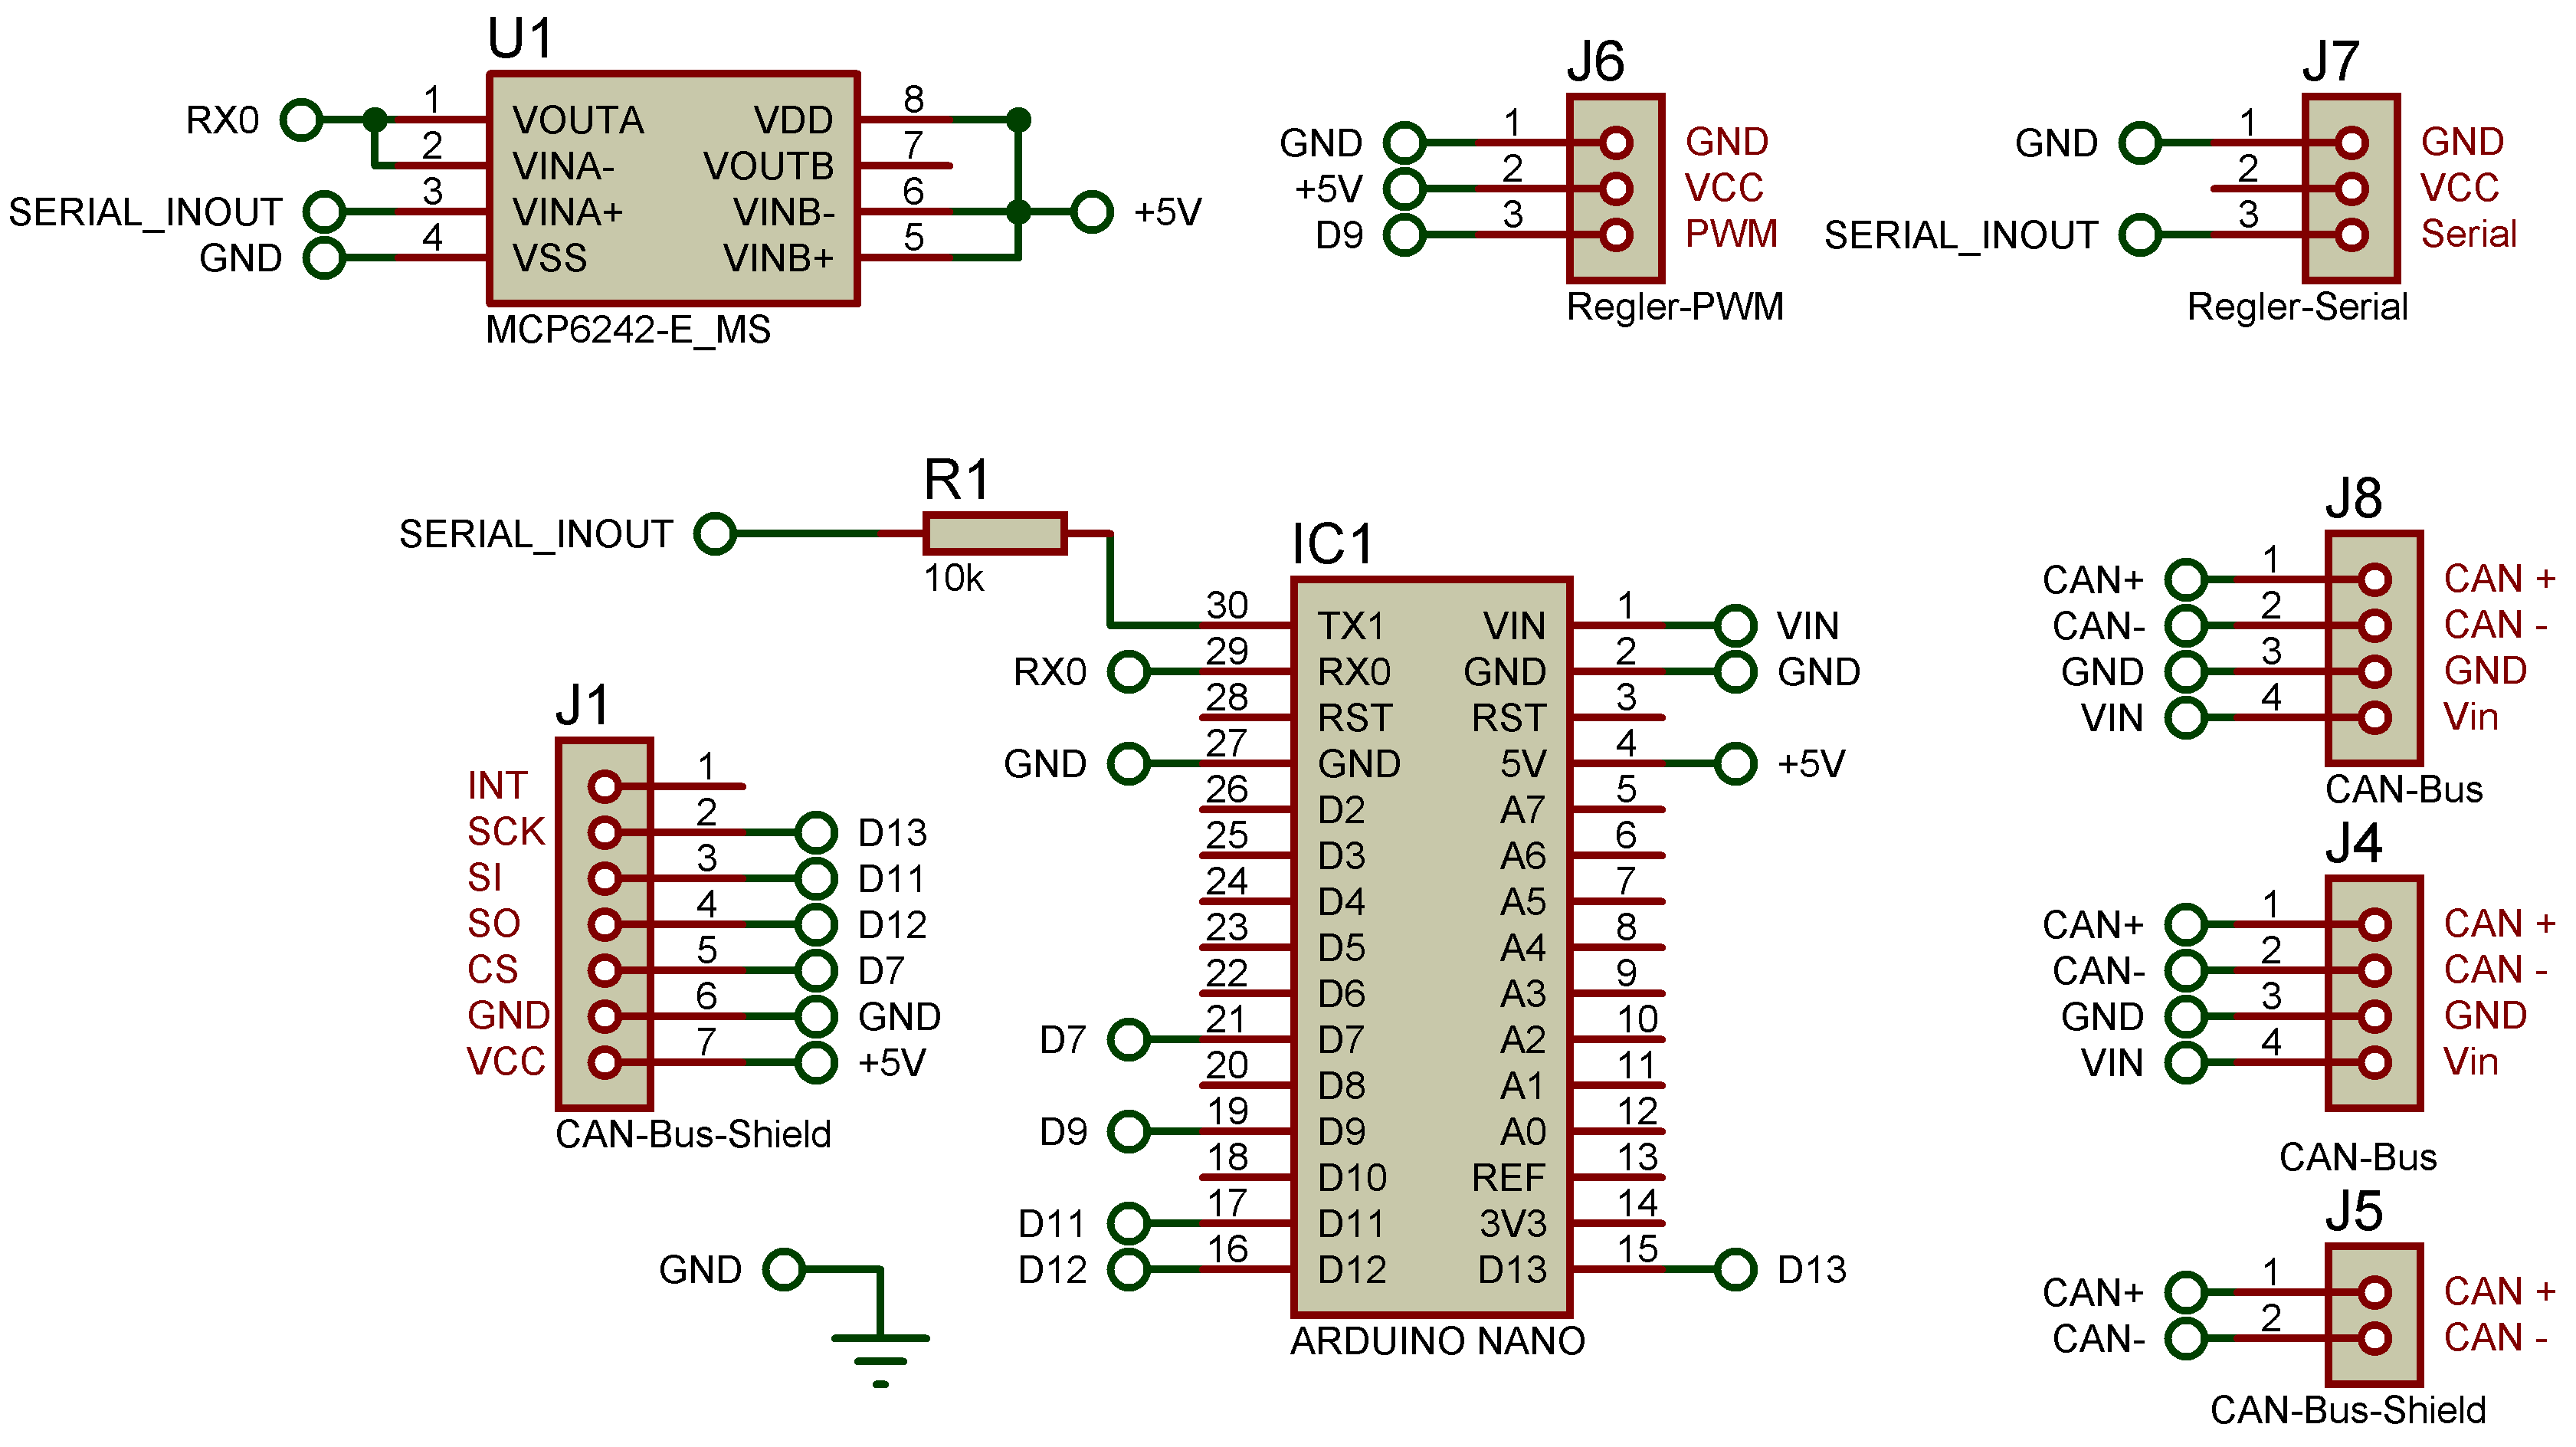
\includegraphics[width=1.0\textwidth]{../Proteus/Exports/Regler-Platine.png}    
    \caption{Schaltplan der Regler-Platine}
\end{figure}

\newpage

\subsubsection{PCB-Layout}
\begin{figure}[h]
    \centering
    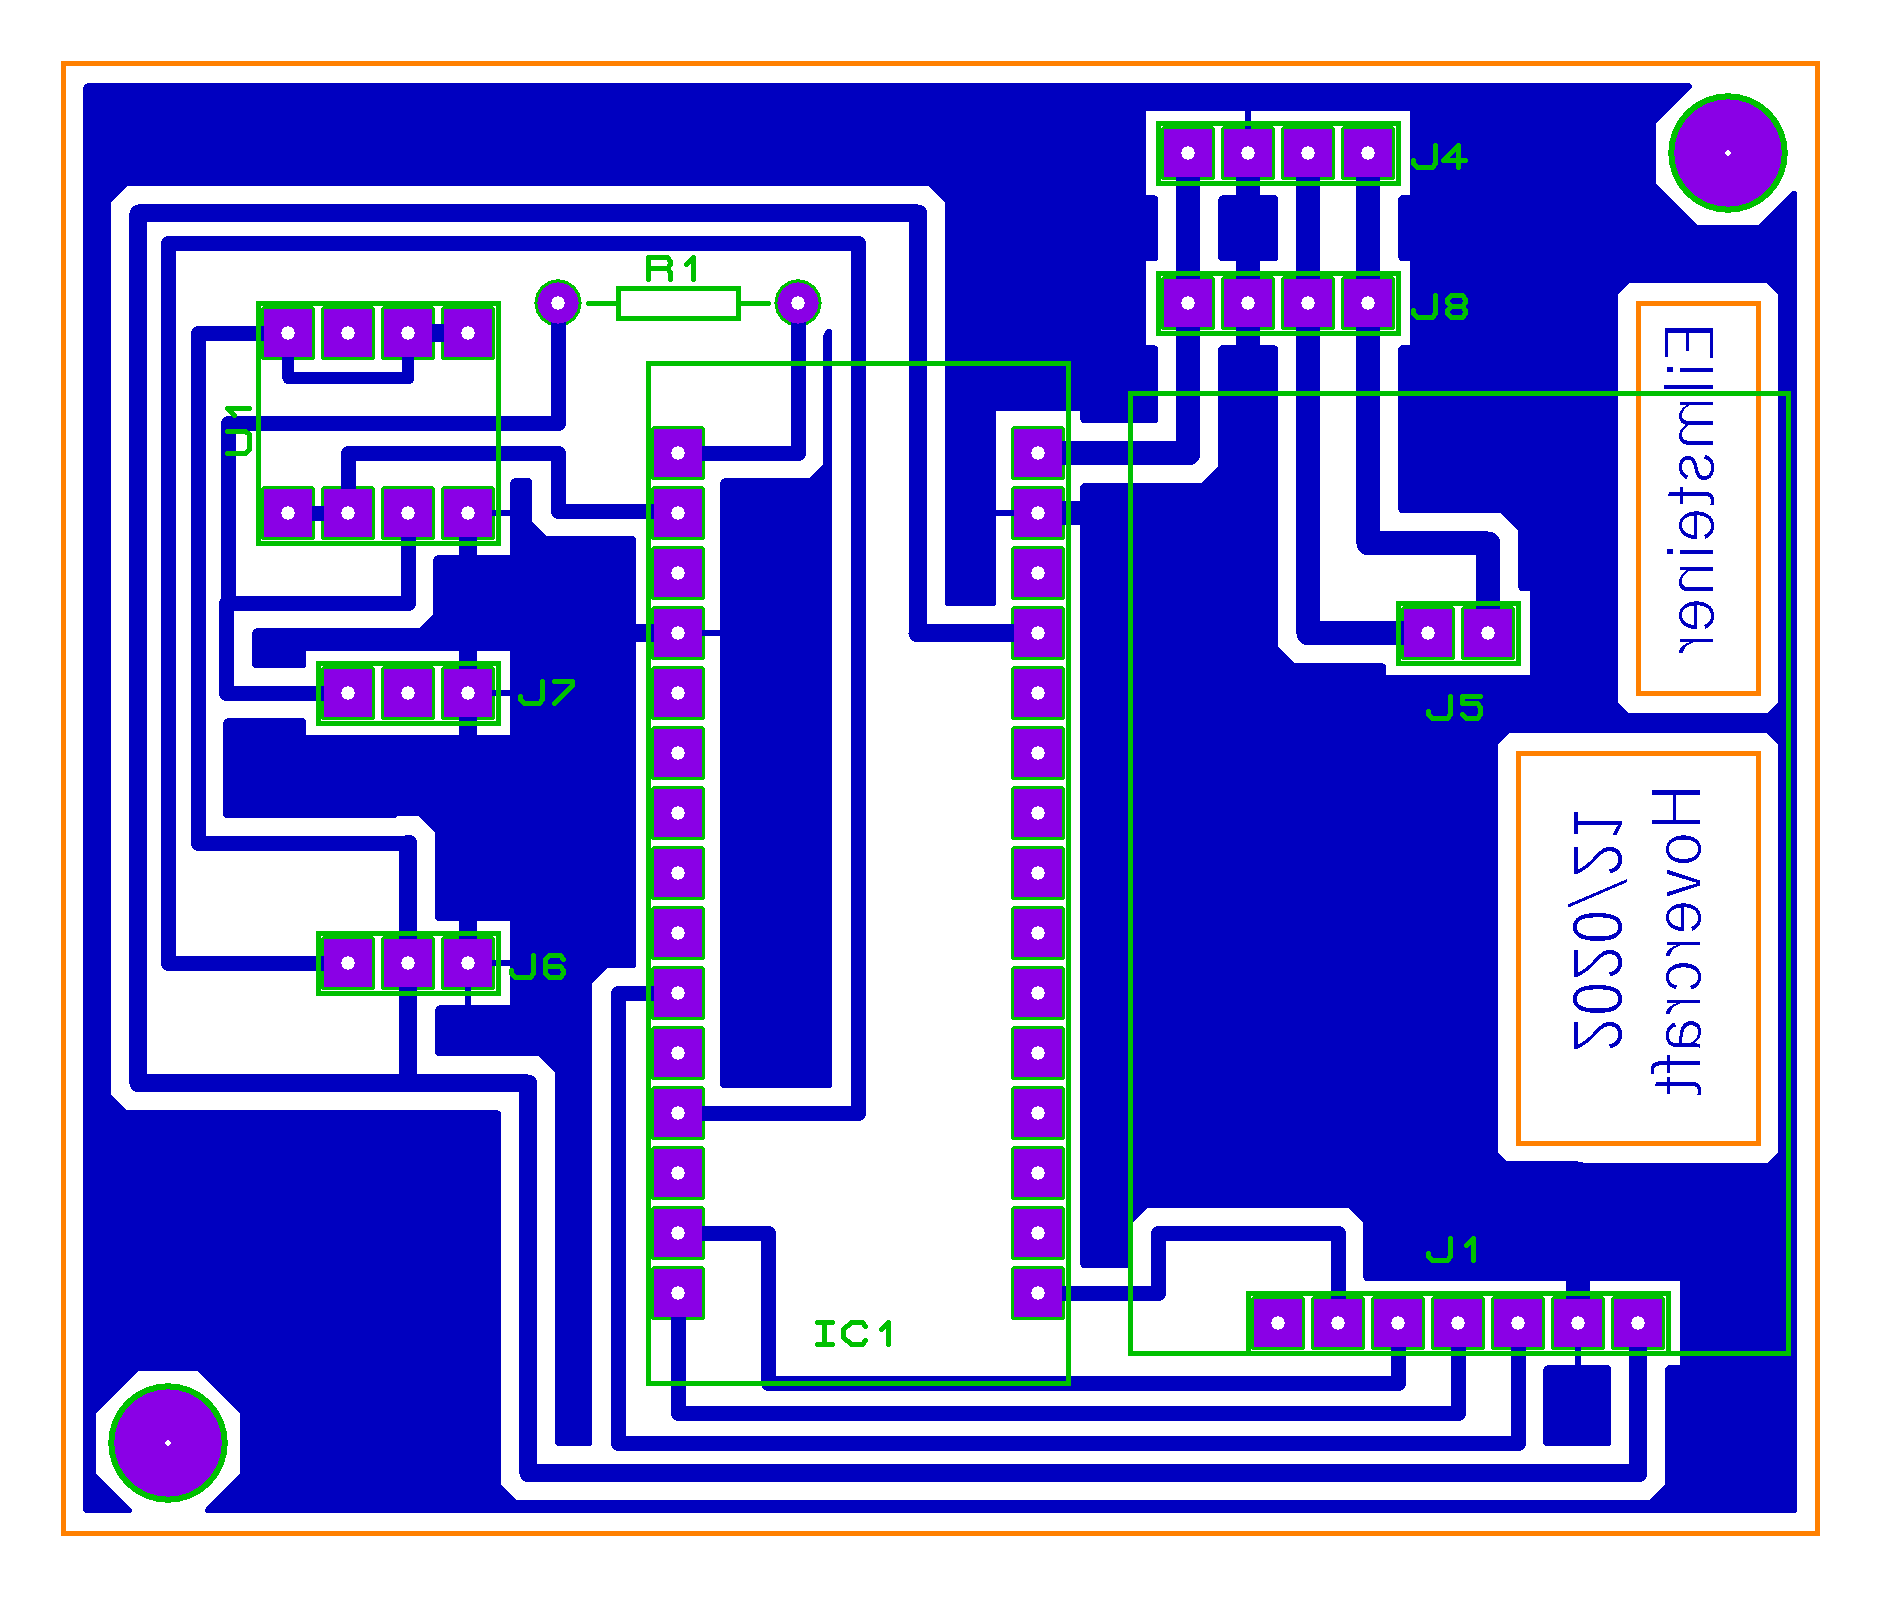
\includegraphics[width=1.0\textwidth]{../Proteus/Exports/Regler_Platine_PCB.png}    
    \caption{Schaltplan der Regler-Platine}
\end{figure}

\newpage
\subsubsection{Programmcode}
\lstinputlisting{../Programmierung/Regler_Controller/src/main.cpp}
\newpage
\subsection{Lenker}
\subsubsection{Aufgaben \& verwendete Bauteile}
Neben seiner Hauptaufgabe, nämlich dem Einlesen und der Übertragung der beiden Daumengas- sowie Lenkerstellungen ist dieser Mikrocontroller weiters für die Darstellung der von den verschiedenen Komponenten erhaltenen Telemetriedaten auf dem Bildschirm verantwortlich.
Dazu zählen neben den Informationen über die beiden Motoren vorallem auch die Temperaturen aller verbauten Akkus sowie die per GPS-Modul ermittelte derzeitige Geschwindigkeit.

\begin{minipage}{8.5cm}
    \begin{tikzpicture}
        \node[anchor=south west,inner sep=0] (image) at (0,0) {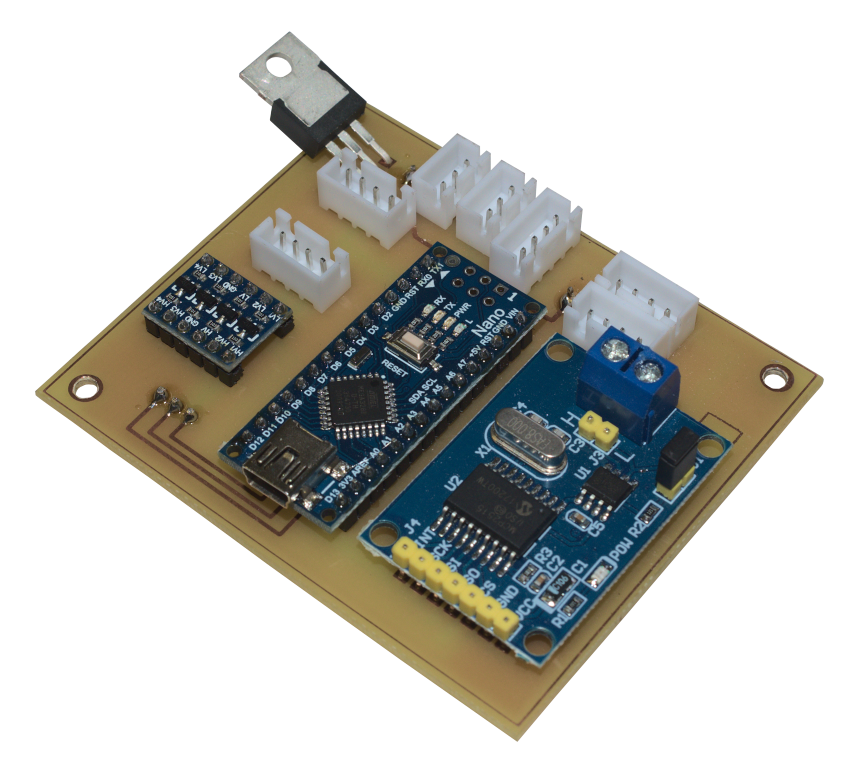
\includegraphics[width=0.9\textwidth]{Fotos/Regler_Lenker.png}};
        \begin{scope}[x={(image.south east)},y={(image.north west)}]
            \draw[red,ultra thick,rounded corners,rotate around={-30:(0.77,0.47)}] (0.6,0.47) rectangle (0.77,0.62);
            \draw[blue,ultra thick,rounded corners,rotate around={-30:(0.4,0.58)}] (0.25,0.58) rectangle (0.4,0.68);
            \draw[orange,ultra thick,rounded corners,rotate around={-30:(0.47,0.67)}] (0.33,0.67) rectangle (0.47,0.76);
            \draw[Green,ultra thick,rounded corners,rotate around={-34:(0.57,0.67)}] (0.45,0.67) rectangle (0.57,0.8);
            \draw[violet,ultra thick,rounded corners,rotate around={-34:(0.62,0.60)}] (0.54,0.60) rectangle (0.62,0.75);
        \end{scope}
    \end{tikzpicture}
    \captionof{figure}{Platine des Lenkers}
\end{minipage}
\begin{minipage}{7cm}
    \textcolor{red}{CAN-Bus Anschlüsse}\\
    \textcolor{blue}{Serielle Verbindung zum GPS-Modul}\\
    \textcolor{orange}{Serielle Verbindung zum Bildschirm}\\
    \textcolor{Green}{Daumengas Anschlüsse}\\
    \textcolor{violet}{Anschluss Lenkerpotenziometer}\\

\end{minipage}

\vspace{0.5cm}
\begin{minipage}{7.5cm}
    \centering
    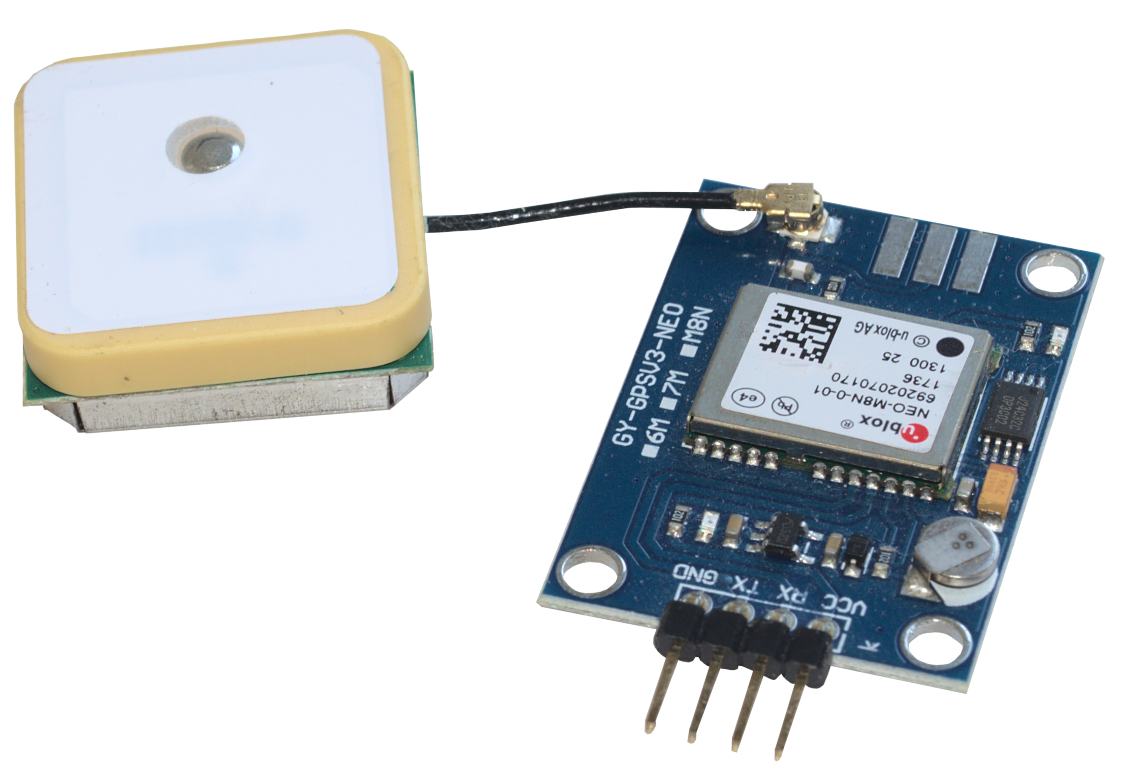
\includegraphics[width=0.99\textwidth]{Fotos/GPS_Modul_2.png}
    \captionof{figure}{NEO-8M GPS-Modul}
\end{minipage}
\hspace{0.1cm}
\begin{minipage}{7.5cm}
    \centering
    \includegraphics[width=0.99\textwidth]{Fotos/Daumengas_2.png}
    \captionof{figure}{Daumengas}
\end{minipage}

\newpage

\subsubsection{Schaltplan}
\begin{figure}[h]
    \centering
    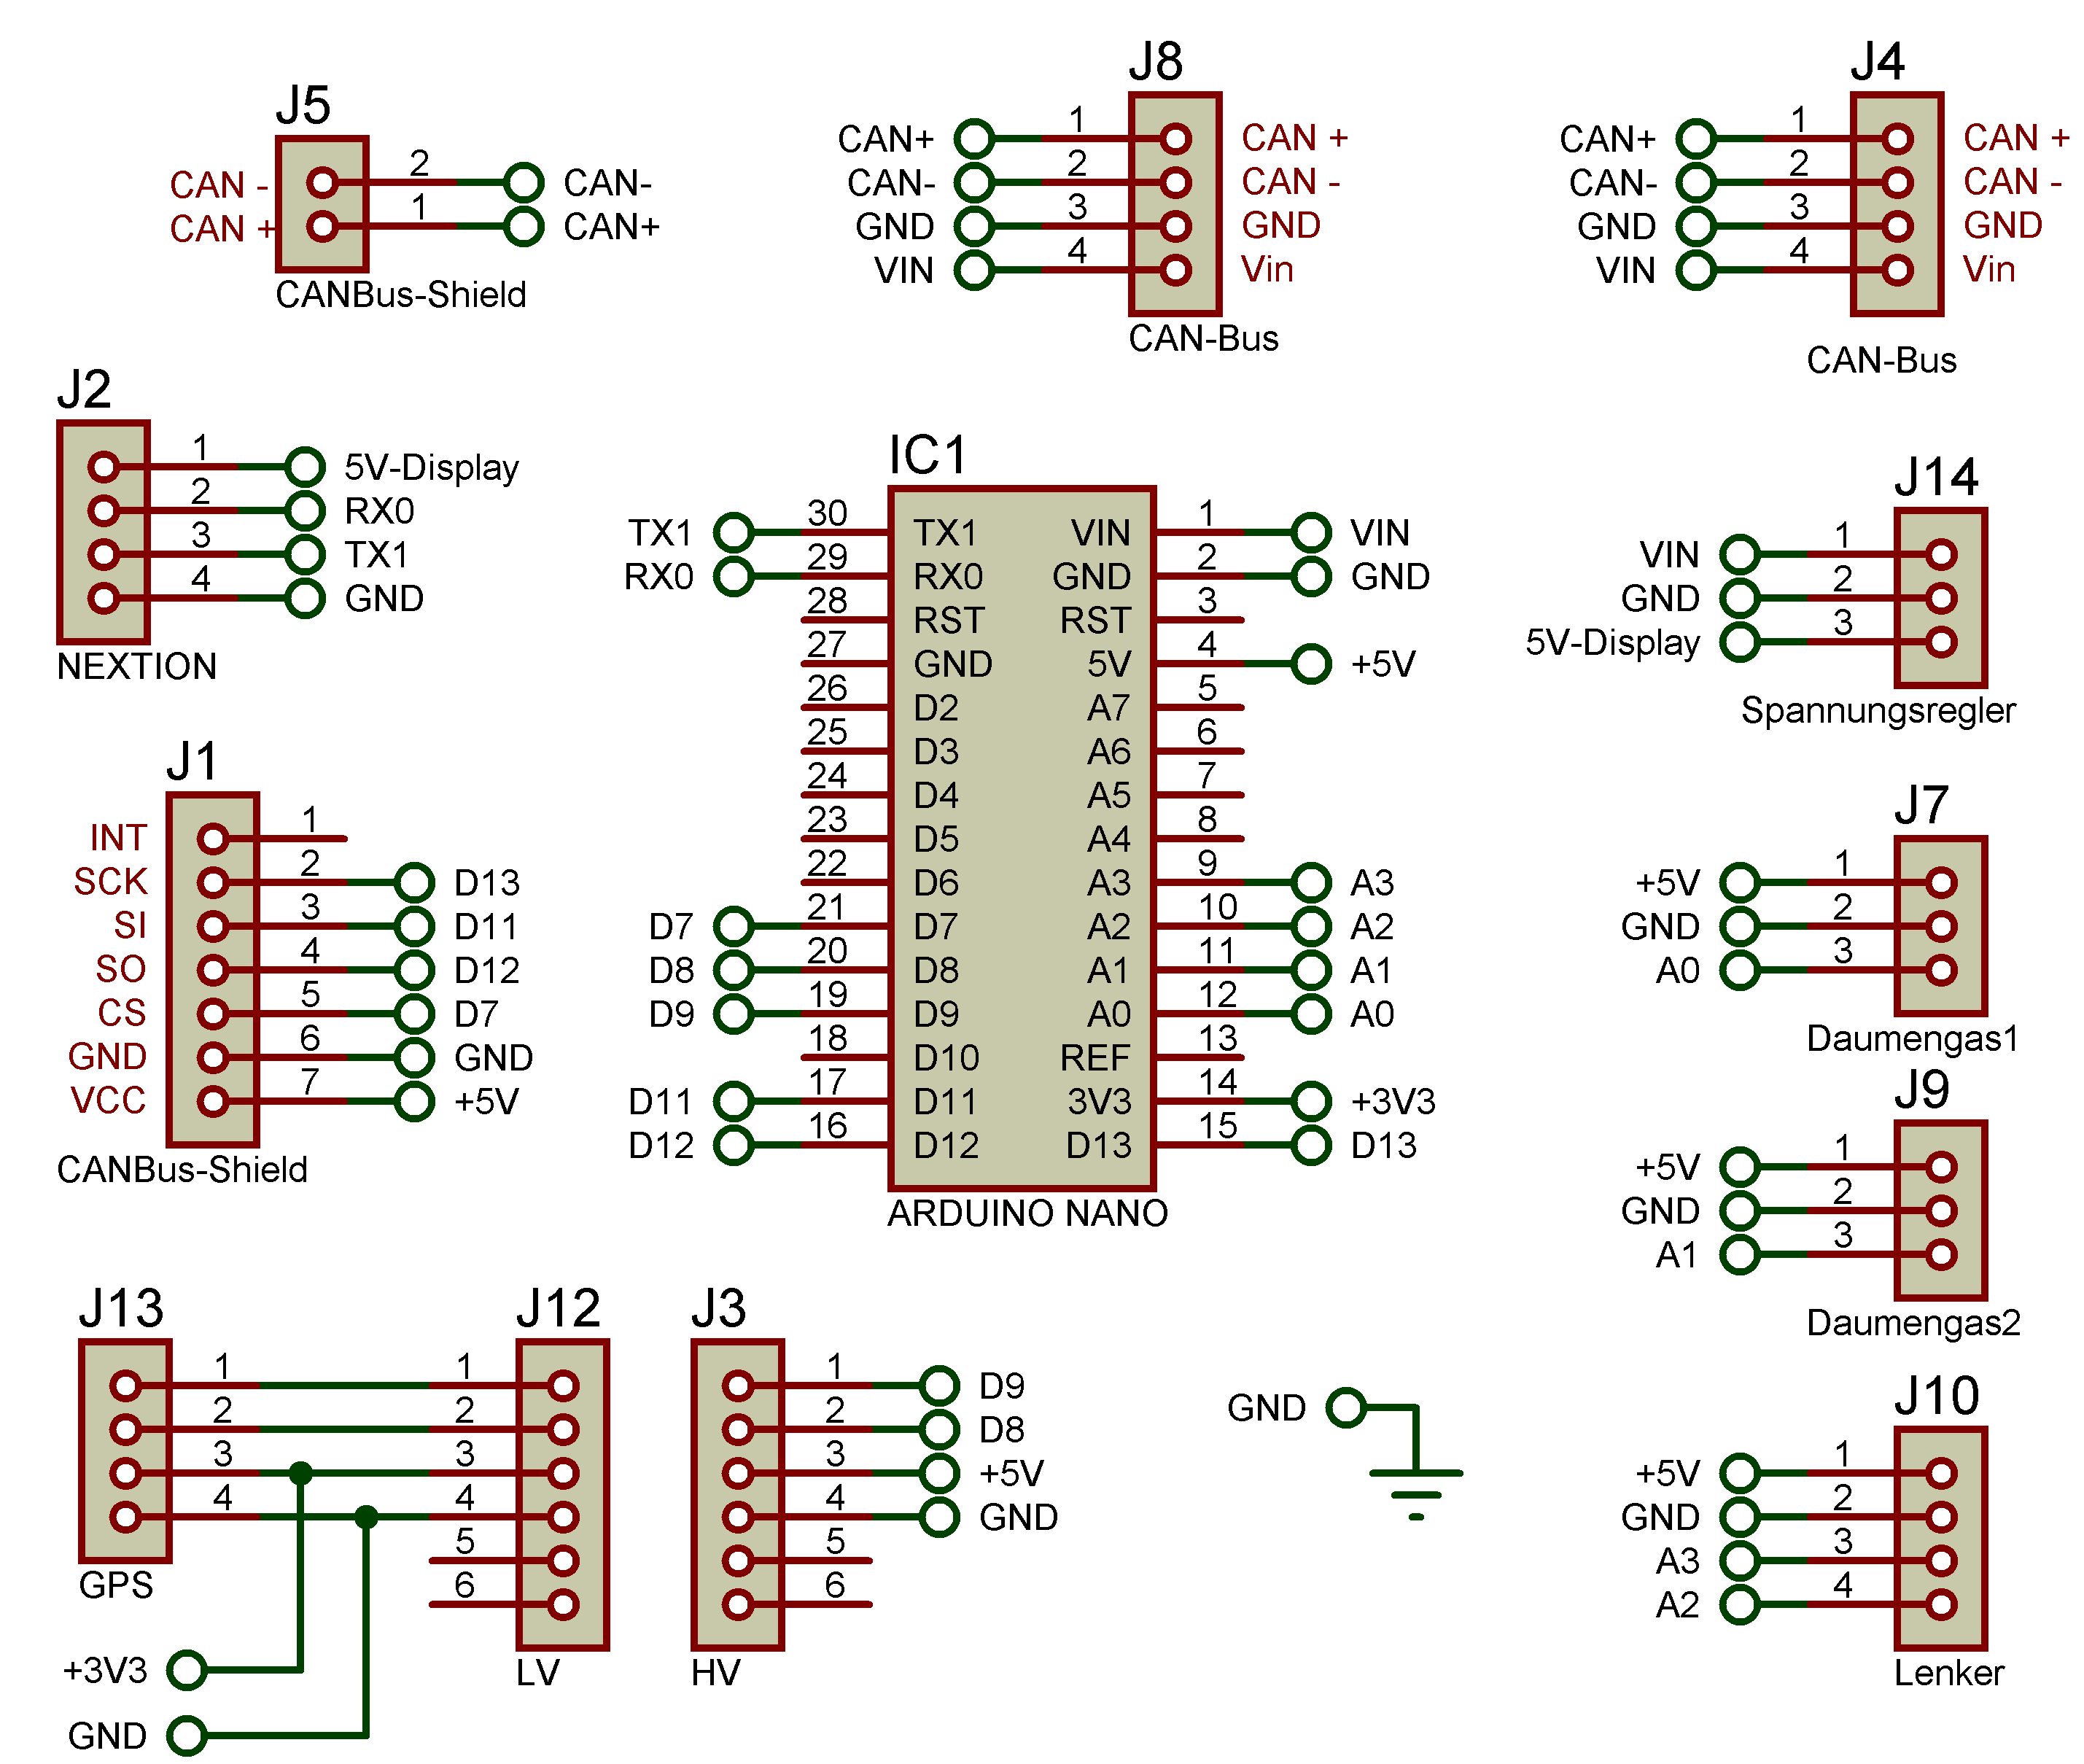
\includegraphics[width=1.0\textwidth]{../Proteus/Exports/Lenker-Platine.png}    
    \caption{Schaltplan der Lenker-Platine}
\end{figure}

\newpage

\subsubsection{PCB-Layout}
\begin{figure}[h]
    \centering
    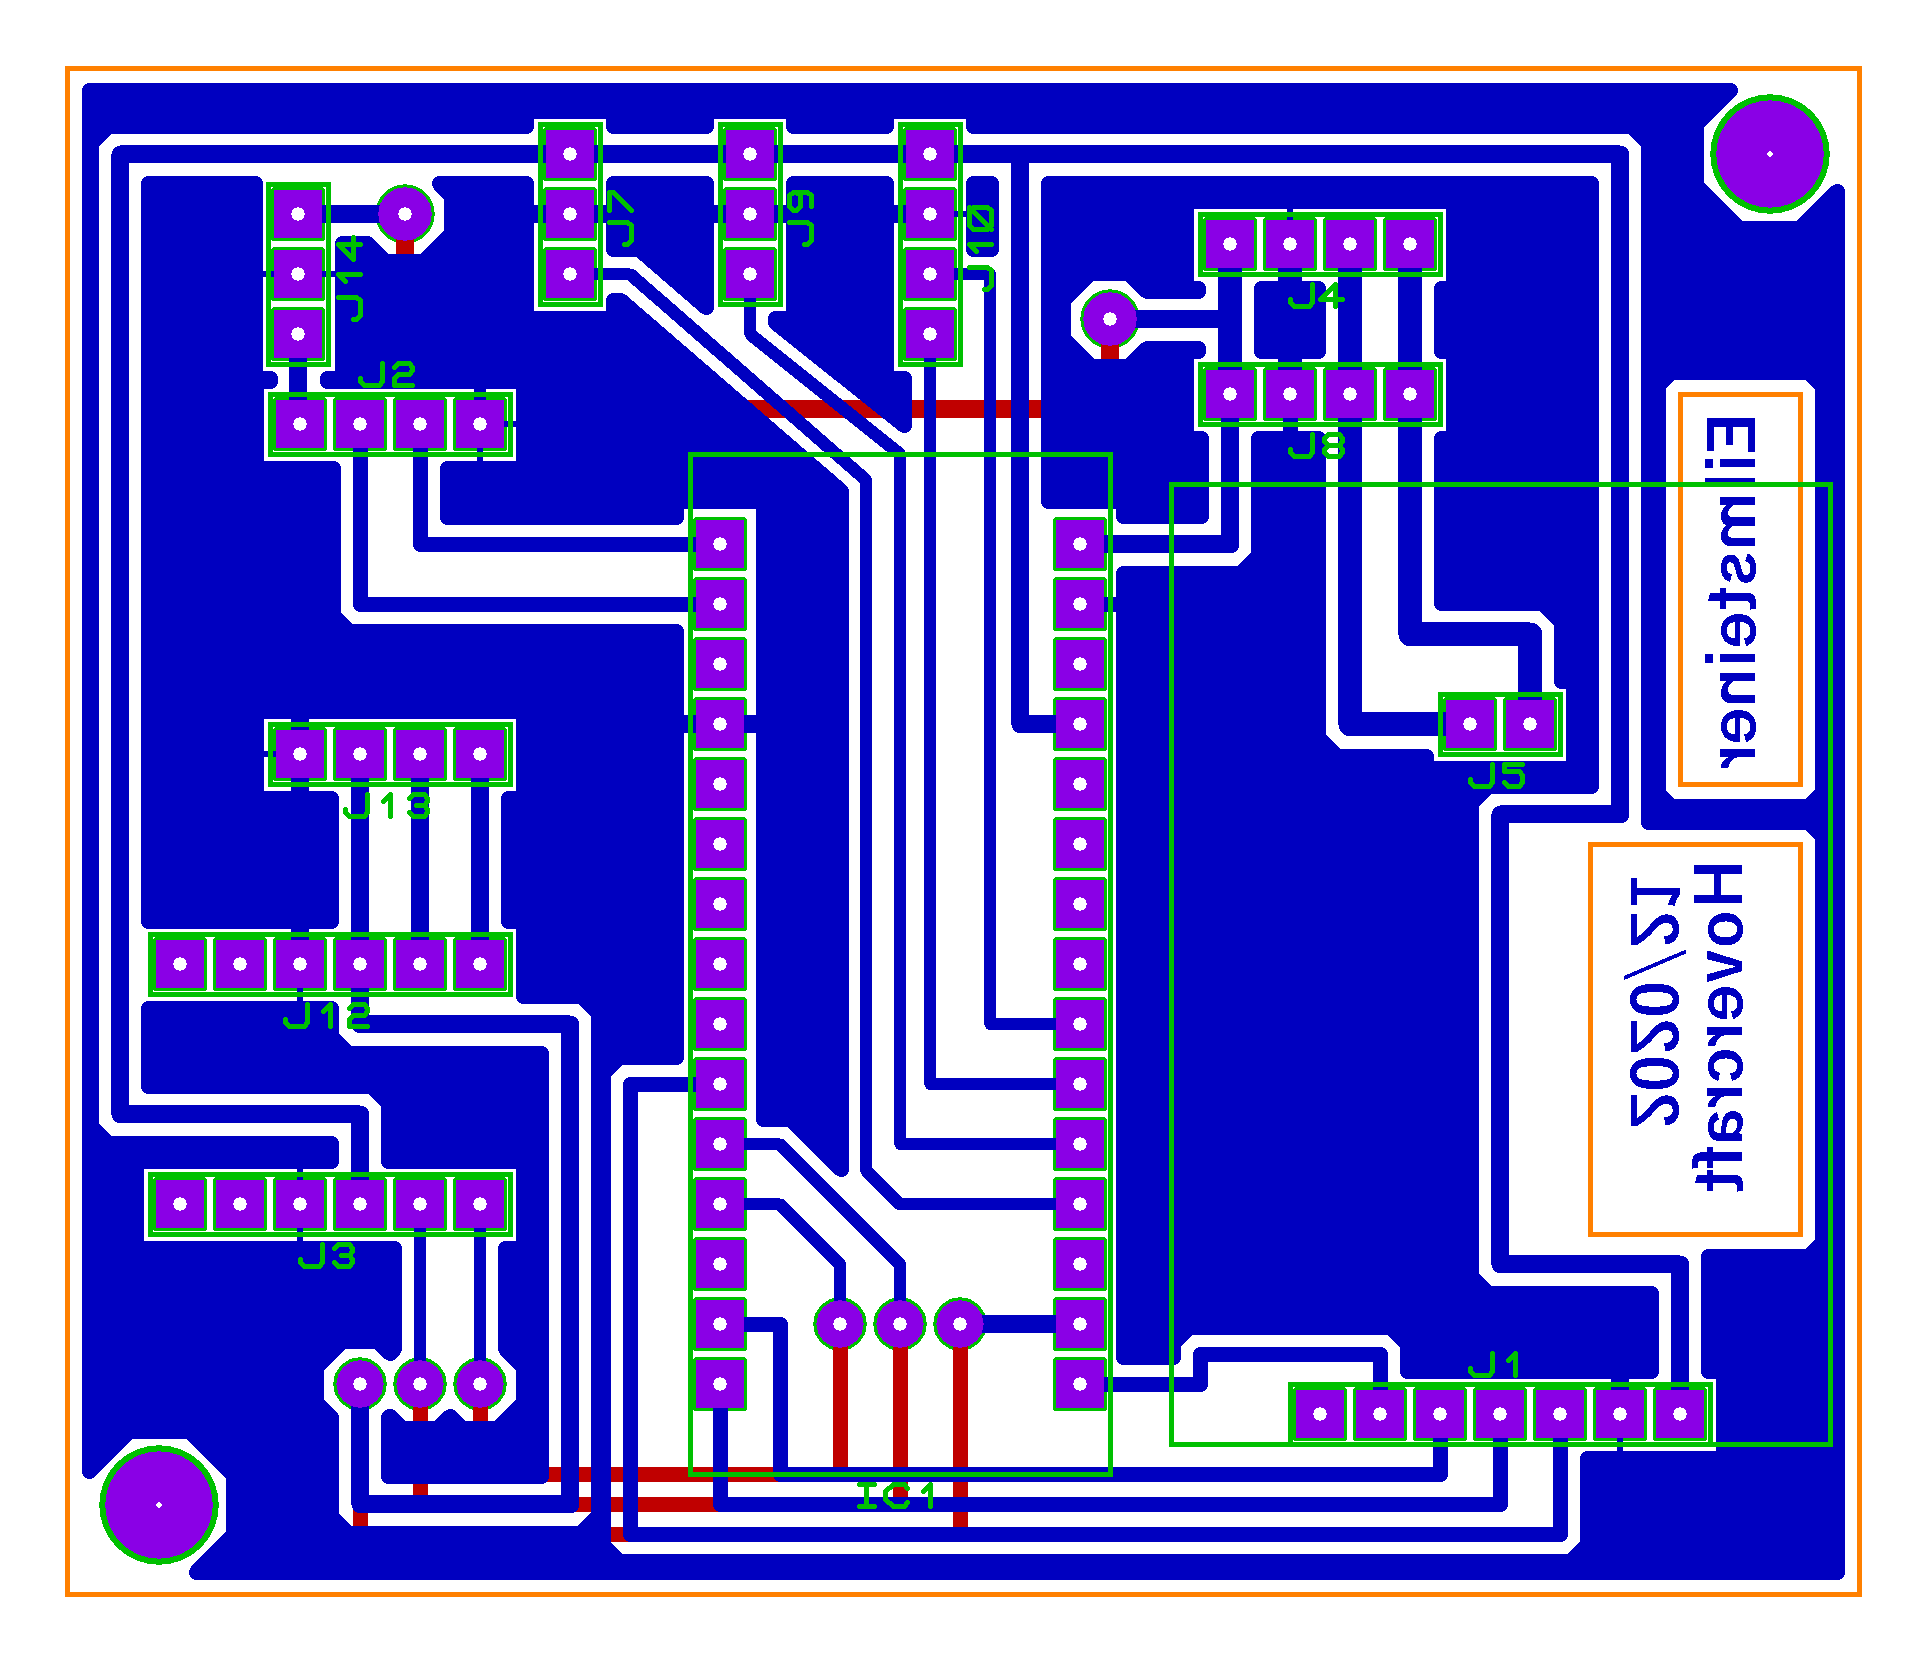
\includegraphics[width=1.0\textwidth]{../Proteus/Exports/Lenker_Platine_PCB.png}    
    \caption{PCB-Layout der Lenker-Platine}
\end{figure}

\newpage
\subsubsection{Programmcode}
\lstinputlisting{../Programmierung/Lenker_Controller/src/main.cpp}

\newpage

\subsection{Fahnenansteuerung \&\ Akkutemperaturen}
\subsubsection{Fahnenansteuerung}
Auch die Ansteuerung der Servos erfolgte mit einem per CAN-Bus angeschlossenen Arduino. Um die für die Steuerung der drei Servos benötigten PWM-Signale unabhängig von den durch den Arduino bereitgestellten Timer und den damit verbunden GPIOs zu erzeugen 
(Anbindung des CAN-Bus Moduls über SPI benötigt beispielsweise diese Pins und Timer), wurde dafür auf ein externes Board zurückgegriffen.

\begin{minipage}{8.5cm}
    \begin{tikzpicture}
        \node[anchor=south west,inner sep=0] (image) at (0,0) {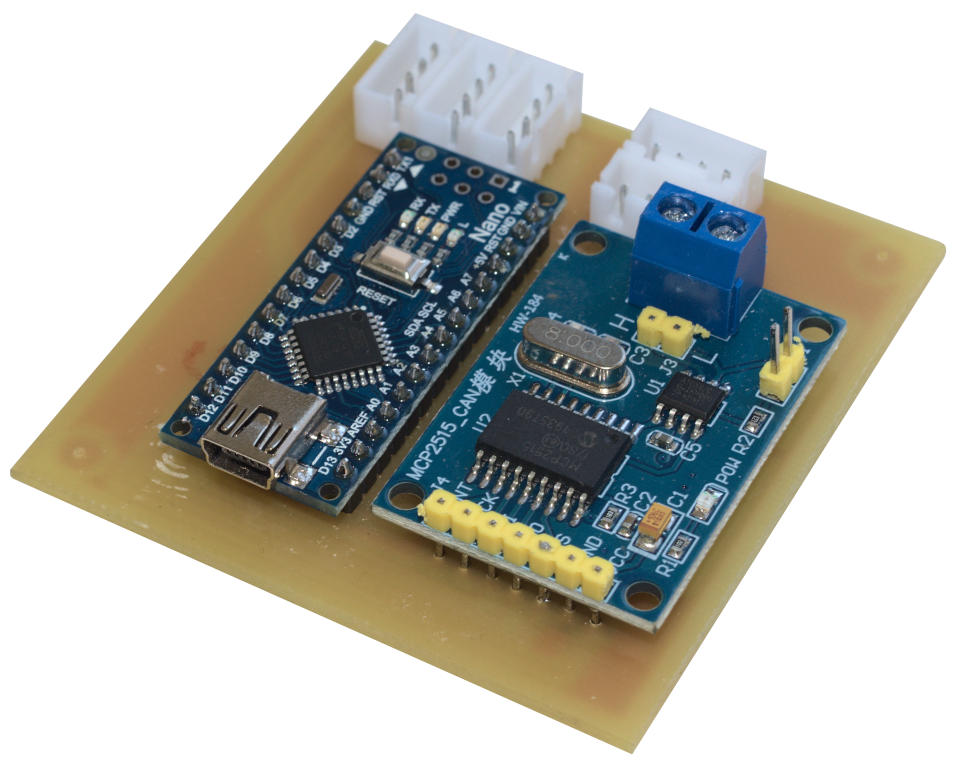
\includegraphics[width=0.9\textwidth]{Fotos/Regler_Servos.png}};
        \begin{scope}[x={(image.south east)},y={(image.north west)}]
            \draw[red,ultra thick,rounded corners,rotate around={-23:(0.64,0.68)}] (0.58,0.67) rectangle (0.78,0.9);
            \draw[blue,ultra thick,rounded corners,rotate around={-20:(0.5,0.9)}] (0.37,0.76) rectangle (0.63,0.99);
        \end{scope}
    \end{tikzpicture}
    \captionof{figure}{Platine zur Regleransteuerung}
\end{minipage}
\begin{minipage}{7cm}
    \textcolor{red}{CAN-Bus Anschlüsse}\\
    \textcolor{blue}{I2C Anschlüsse}\\
    
\end{minipage}\\

Konkret handelt es sich um das \textbf{16-Channel 12-bit PWM/Servo Driver Module} von Adafruit, welcher mittels I2C mit dem Mikrocontroller kommuniziert.\\
\begin{figure}[h]
    \centering
    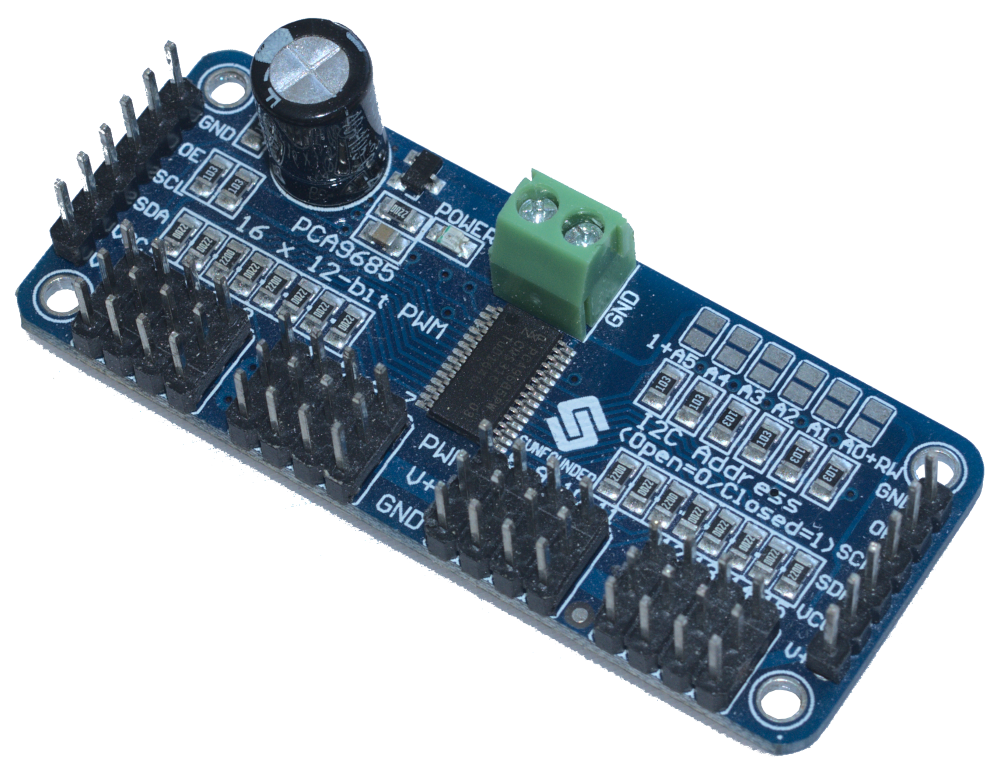
\includegraphics[width=0.5\textwidth]{Fotos/Servo_Controller.png}
    \caption{Adafruit 16-Channel Servo Driver}
\end{figure}

\newpage
\subsubsection{Schaltplan}
\begin{figure}[h]
    \centering
    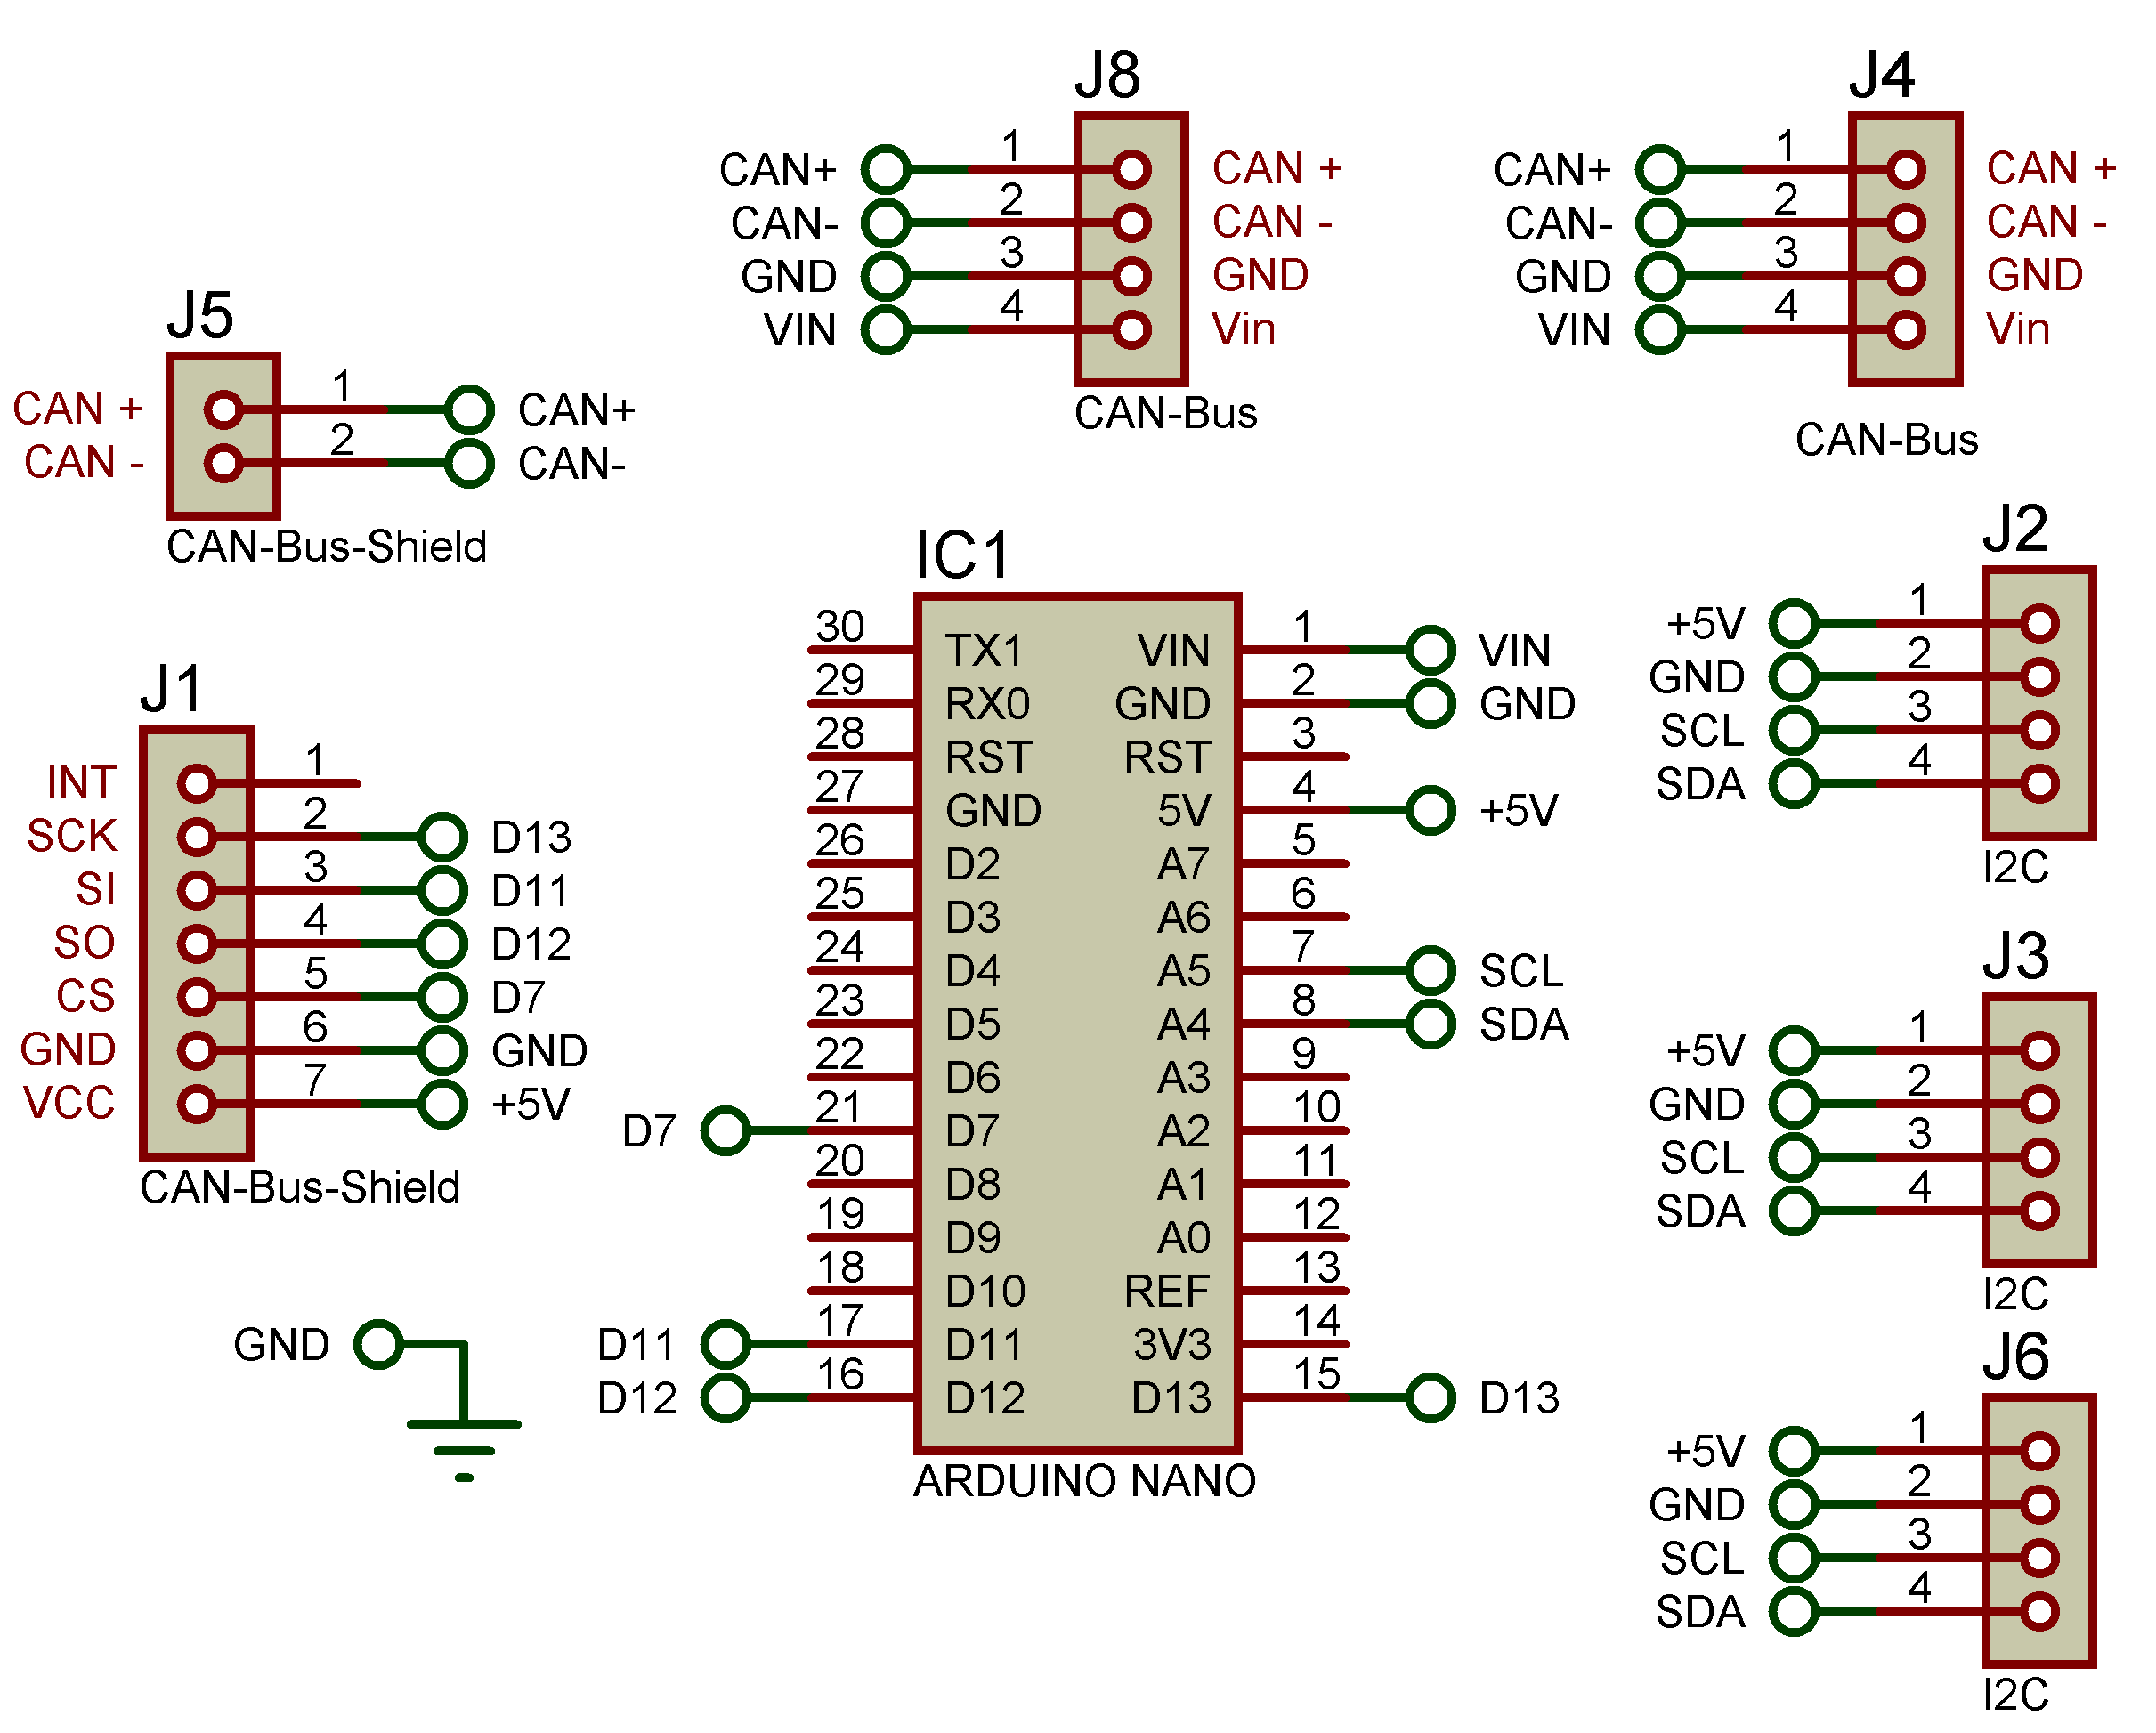
\includegraphics[width=1.0\textwidth]{../Proteus/Exports/Servos-Platine.png}    
    \caption{Schaltplan der Servoansteuerung-Platine}
\end{figure}

\newpage
\subsubsection{PCB-Layout}
\begin{figure}[h]
    \centering
    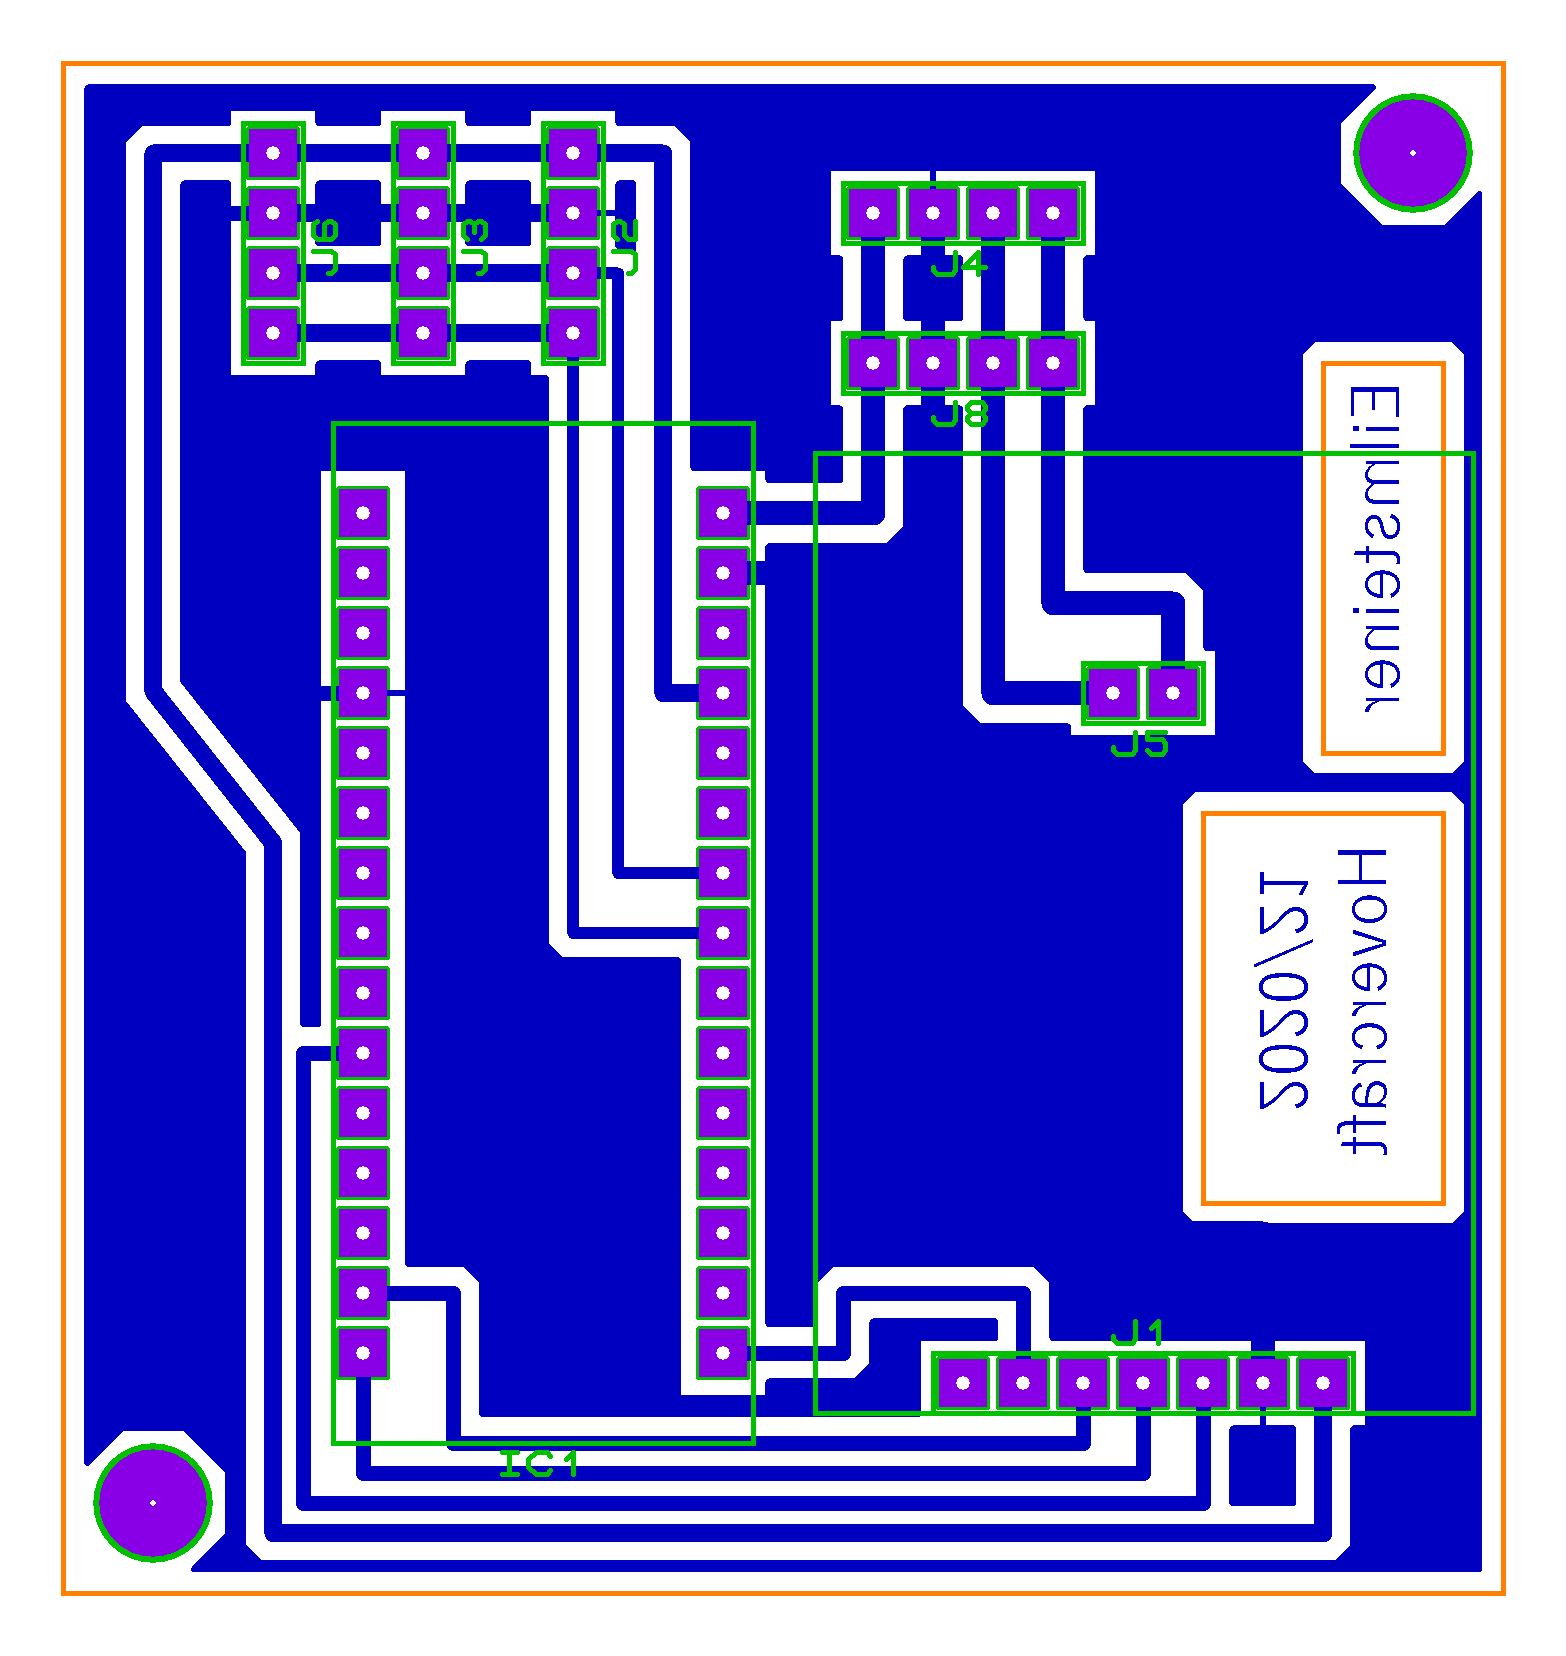
\includegraphics[width=0.9\textwidth]{../Proteus/Exports/Servos-Platine-PCB.png}    
    \caption{PCB-Layout der Servoansteuerung-Platine}
\end{figure}

\newpage
\subsubsection{Programmcode}
\lstinputlisting{../Programmierung/Servo_ADC_Controller/src/main.cpp}
\newpage

\subsubsection{Akkutemperaturen}
Die zweite Aufgabe dieses Controllers ist es, die Temperaturen aller acht im Boot verbauten Akkus zu überwachen, und diese zur Darstellung an den Controller des Lenkers zu übermitteln.
Dies geschieht mithilfe zweier (je einer pro Seite verbauten) ebenfalls über I2C verbundenen \textbf{ADS1115} Analog-Digital-Wandler, welche wiederum von Adafruit stammen.\\
Zur Temperaturmessung selbst kommt je ein \textbf{LM35} Temperatursensor pro Akku zum Einsatz.\\

\begin{minipage}{8cm}
    \centering
    \includegraphics[width=0.85\textwidth]{Fotos/ADS1115_2.png}
    \captionof{figure}{ADS1115 Modul}    
\end{minipage}
\begin{minipage}{8cm}
    \centering
    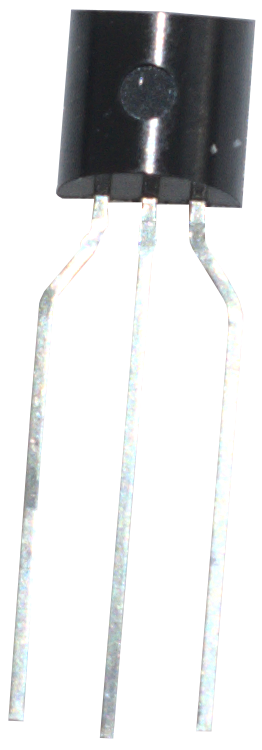
\includegraphics[width=0.17\textwidth]{Fotos/LM35.png}
    \captionof{figure}{LM35}
\end{minipage}\\
\vspace{0.5cm}

\subsection{ADC-Platinen}
Um den Anschluss der Temperatursensoren an diesem ADC zu vereinfachen, wurde folgende Platine entworfen:\\ 
\begin{minipage}{9cm}
    \begin{tikzpicture}
        \node[anchor=south west,inner sep=0] (image) at (0,0) {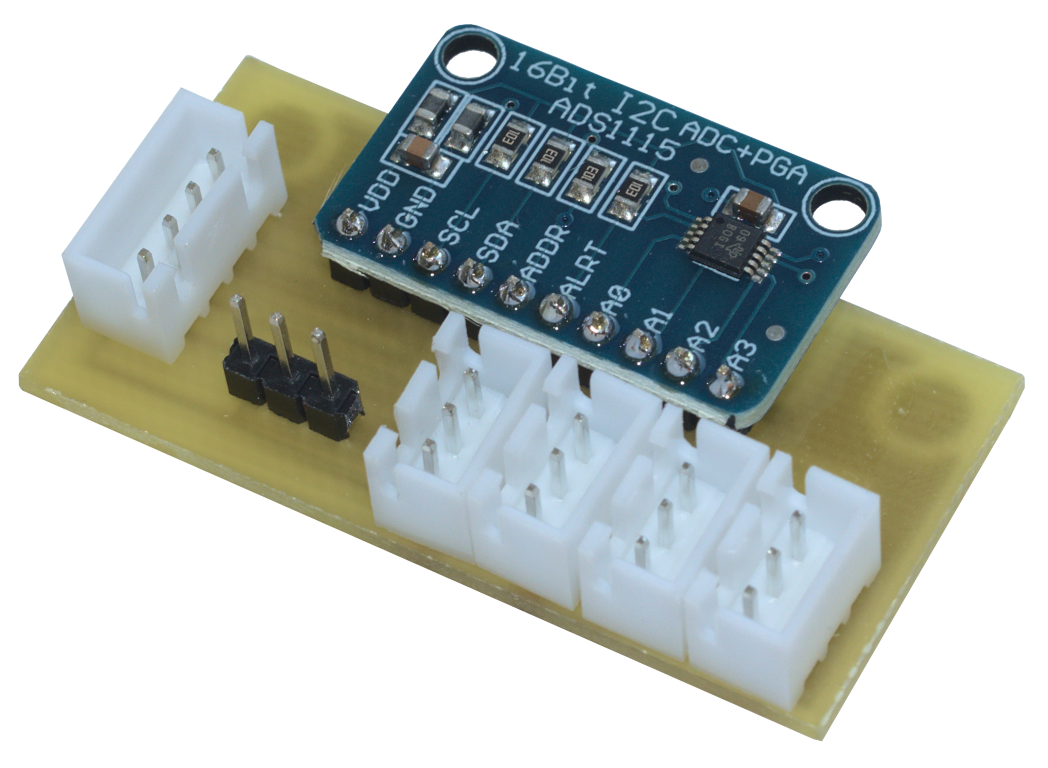
\includegraphics[width=0.9\textwidth]{Fotos/ADC_Platine.png}};
        \begin{scope}[x={(image.south east)},y={(image.north west)}]
            \draw[red,ultra thick,rounded corners,rotate around={-23:(0.78,0.0)}] (0.25,0.0) rectangle (0.78,0.4);
            \draw[blue,ultra thick,rounded corners,,rotate around={-30:(0.00,0.59)}] (0.00,0.59) rectangle (0.20,0.99);
            \draw[Green,ultra thick,rounded corners,,rotate around={-27:(0.3,0.4)}] (0.15,0.4) rectangle (0.34,0.57);
        \end{scope}
    \end{tikzpicture}
    \captionof{figure}{Platine Temperatursensoren}
\end{minipage}
\begin{minipage}{7cm}
    \textcolor{red}{Analogeingänge}\\
    \textcolor{blue}{I2C Anschluss}\\
    \textcolor{Green}{I2C Adressen-Jumper}\\
\end{minipage}\\

\newpage
\subsubsection{Schaltplan}
\begin{figure}[h]
    \centering
    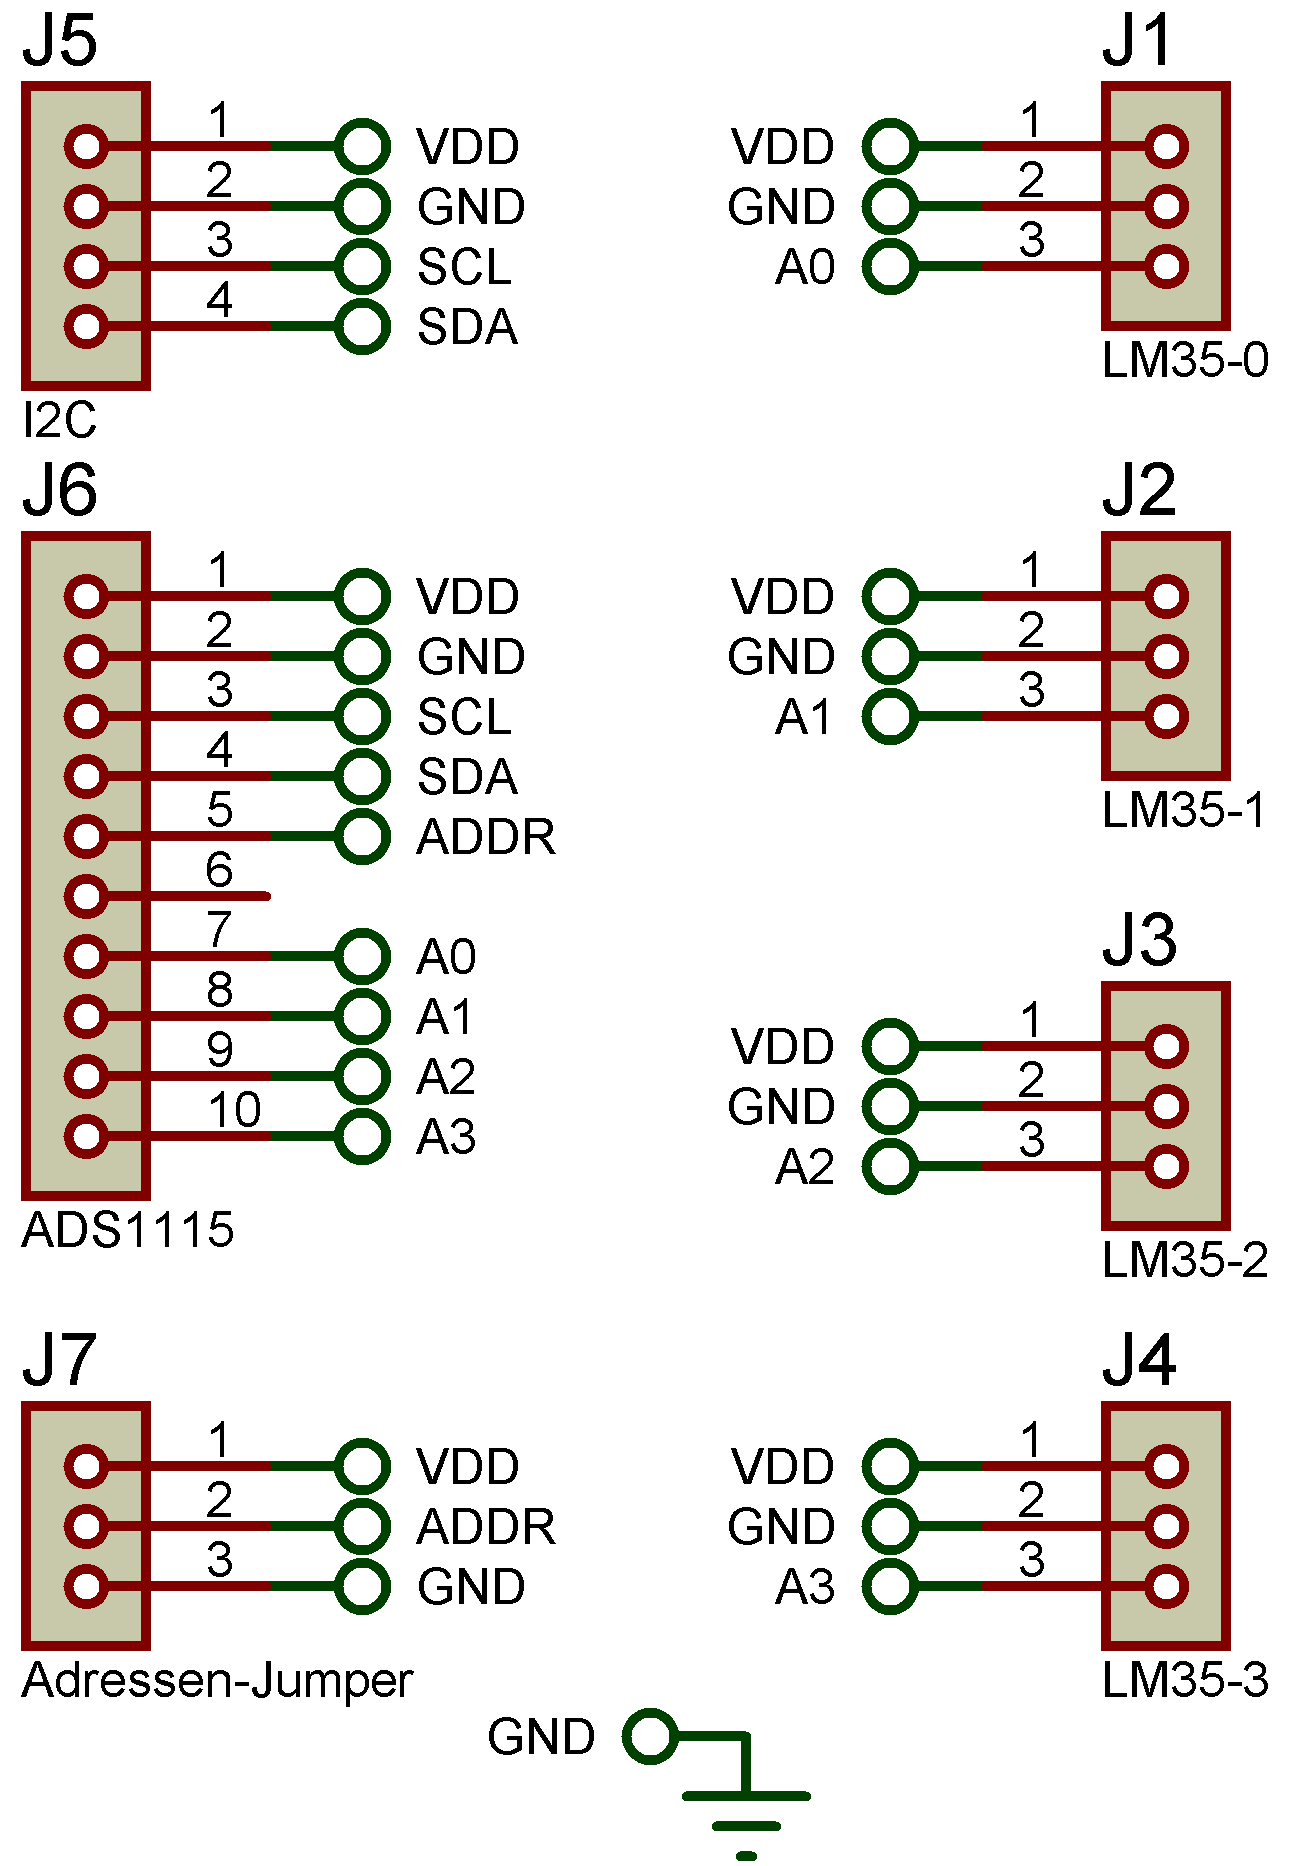
\includegraphics[width=0.6\textwidth]{../Proteus/Exports/Temperatursensoren-Platine.png}    
    \caption{Schaltplan der Temperatursensoren-Platine}
\end{figure}

\newpage

\subsubsection{PCB-Layout}
\begin{figure}[h]
    \centering
    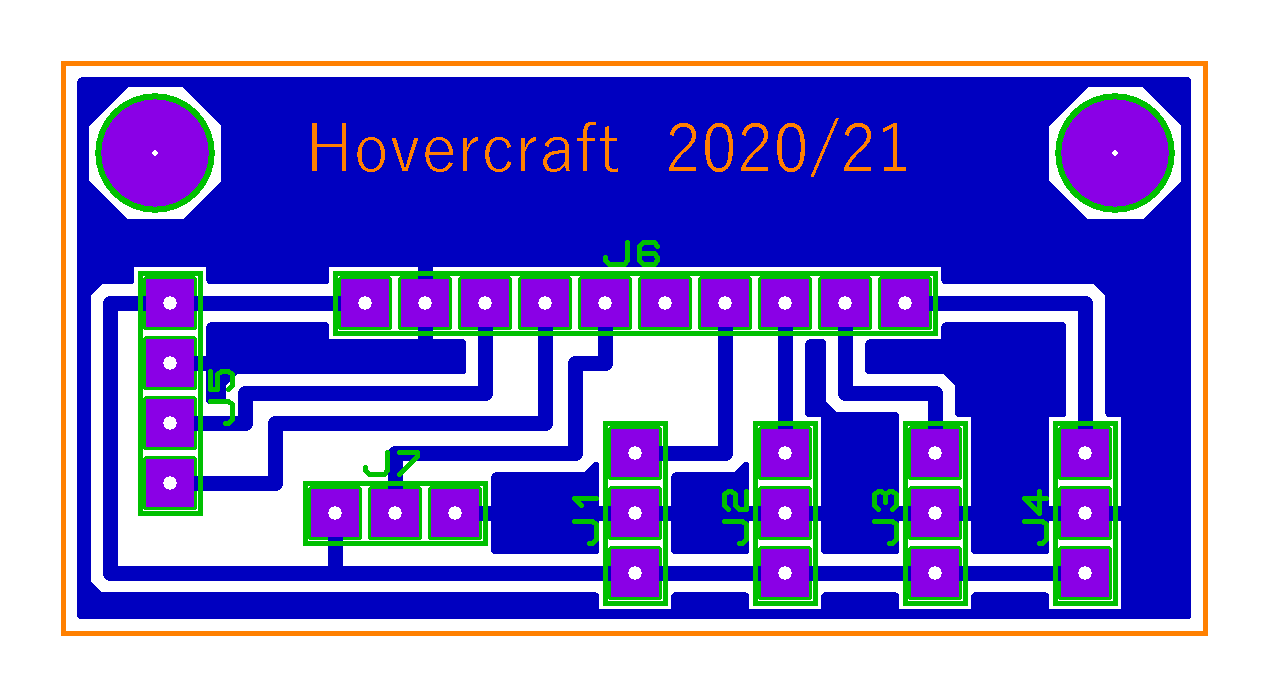
\includegraphics[width=0.8\textwidth]{../Proteus/Exports/Temperatursensoren-Platine-PCB.png}    
    \caption{PCB-Layout der Temperatursensoren-Platine}
\end{figure}

\newpage
\subsection{Precharge \& Relaisansteuerung}
Da sowohl die Motorregler als auch die Buck-Converter einen, durch die darin verbauten sehr großen Kondensatoren bedingten, sehr großen Einschaltstrom haben, 
müssen diese über einen Leistungswiderstand vorgeladen werden, bevor sie permanent mit Spannung versorgt werden können.\\
\begin{figure}[h]
    \centering
    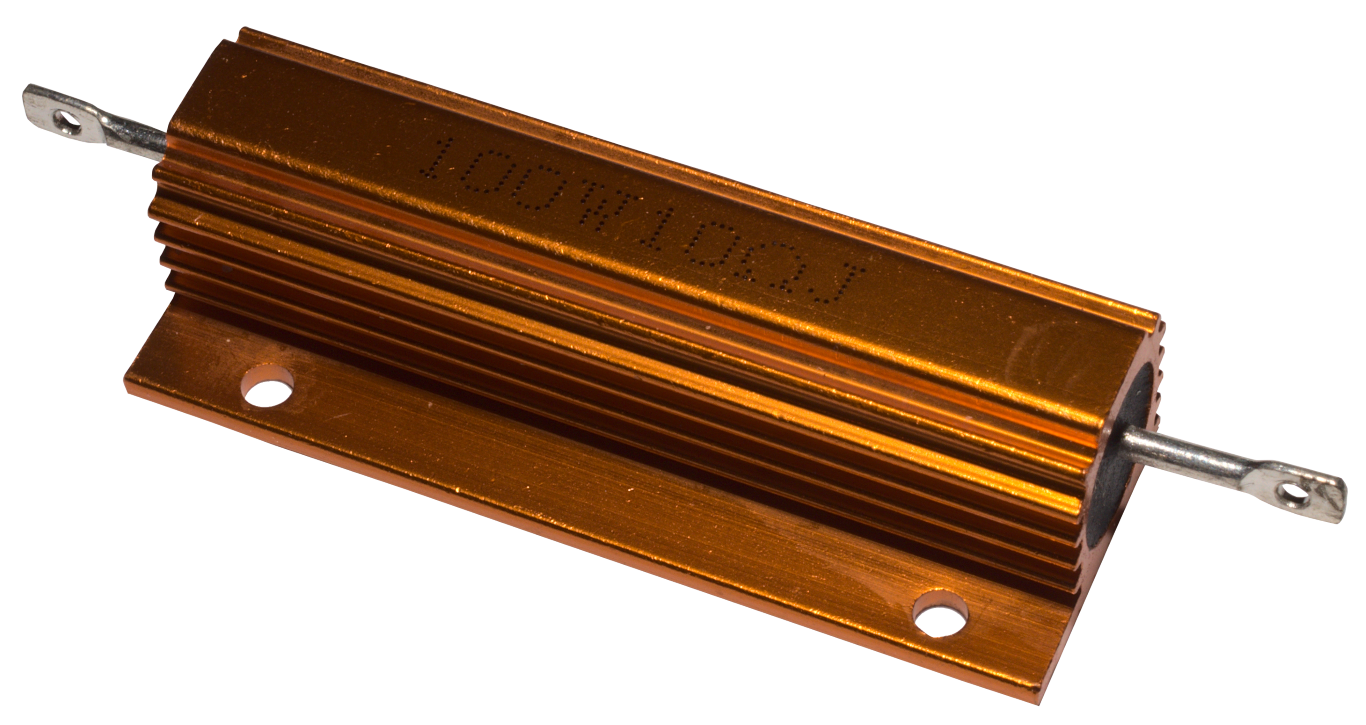
\includegraphics[width=0.55\textwidth]{Fotos/Leistungswiderstand.png}
    \caption{Zur Vorladung verwendeter Leistungswiderstand}
\end{figure}

Um diese Umschaltung so einfach wie möglich zu gestalten, wurde dies mithilfe einer im folgenden genauer erläuterten Platine realisiert. 

\begin{minipage}{9cm}
    \begin{tikzpicture}
        \node[anchor=south west,inner sep=0] (image) at (0,0) {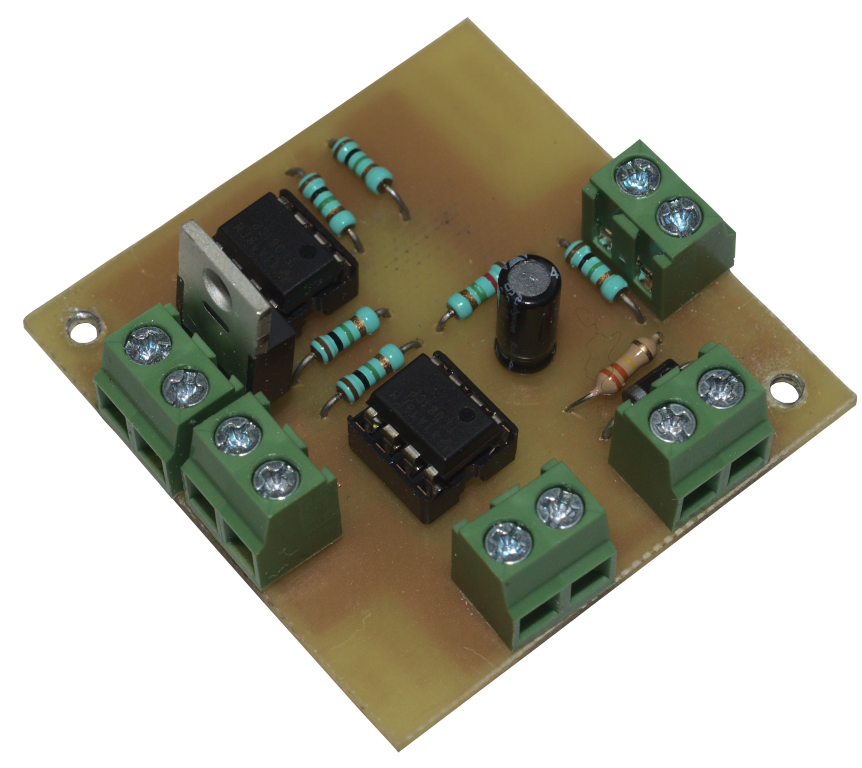
\includegraphics[width=0.9\textwidth]{Fotos/Platine_Relaischaltung.png}};
        \begin{scope}[x={(image.south east)},y={(image.north west)}]
            \draw[red,ultra thick,rounded corners,rotate around={30:(0.58,0.11)}] (0.58,0.11) rectangle (0.79,0.35);
            \draw[blue,ultra thick,rounded corners,rotate around={30:(0.77,0.28)}] (0.77,0.28) rectangle (0.97,0.51);
            \draw[orange,ultra thick,rounded corners,rotate around={37:(0.29,0.21)}] (0.29,0.21) rectangle (0.46,0.42);
            \draw[Green,ultra thick,rounded corners,rotate around={37:(0.16,0.38)}] (0.16,0.38) rectangle (0.34,0.55);
            \draw[violet,ultra thick,rounded corners,rotate around={40:(0.78,0.56)}] (0.78,0.56) rectangle (0.93,0.81);
        \end{scope}
    \end{tikzpicture}
    \captionof{figure}{Platine zur Relaisansteuerung}
\end{minipage}
\begin{minipage}{7.5cm}
    \textcolor{Green}{Hauptrelaisspule (A- \& GND)}\\
    \textcolor{blue}{Micro-Switches im Ladedeckel}\\
    \textcolor{orange}{Buck-Converter (nicht verwendet)}\\
    \textcolor{violet}{+30 V von geschalteter Relaisseite}\\
    \textcolor{red}{Konstante +30 V}\\
\end{minipage}\\
\newpage
\subsubsection{Funktionsweise}
Durch das Zusammenschalten der Akkus, über den bereits zuvor gezeigten $10\,\mathrm{\Omega}$ Leistungswiderstand, beginnen sich sowohl die Kondensatoren beider Motorregler, aller vier Buck-Converter sowie jener des sich auf der Platine befindlichen RC-Gliedes aufzuladen.\\
Erreicht dieser eine bestimmte Schwellspannung, wird das Hauptrelais mithilfe eines MOSFETs durch den Operationsverstärker der Komperatorschaltung aktiviert.\\
Dies führt zu einer Selbsthaltung des Relais, welche nur durch Betätigung des NOTAUS-Schalters oder dem Öffnen einer der beiden Mikroschalter unterbrochen werden kann.
\subsubsection{Schaltplan}
\begin{figure}[h]
    \centering
    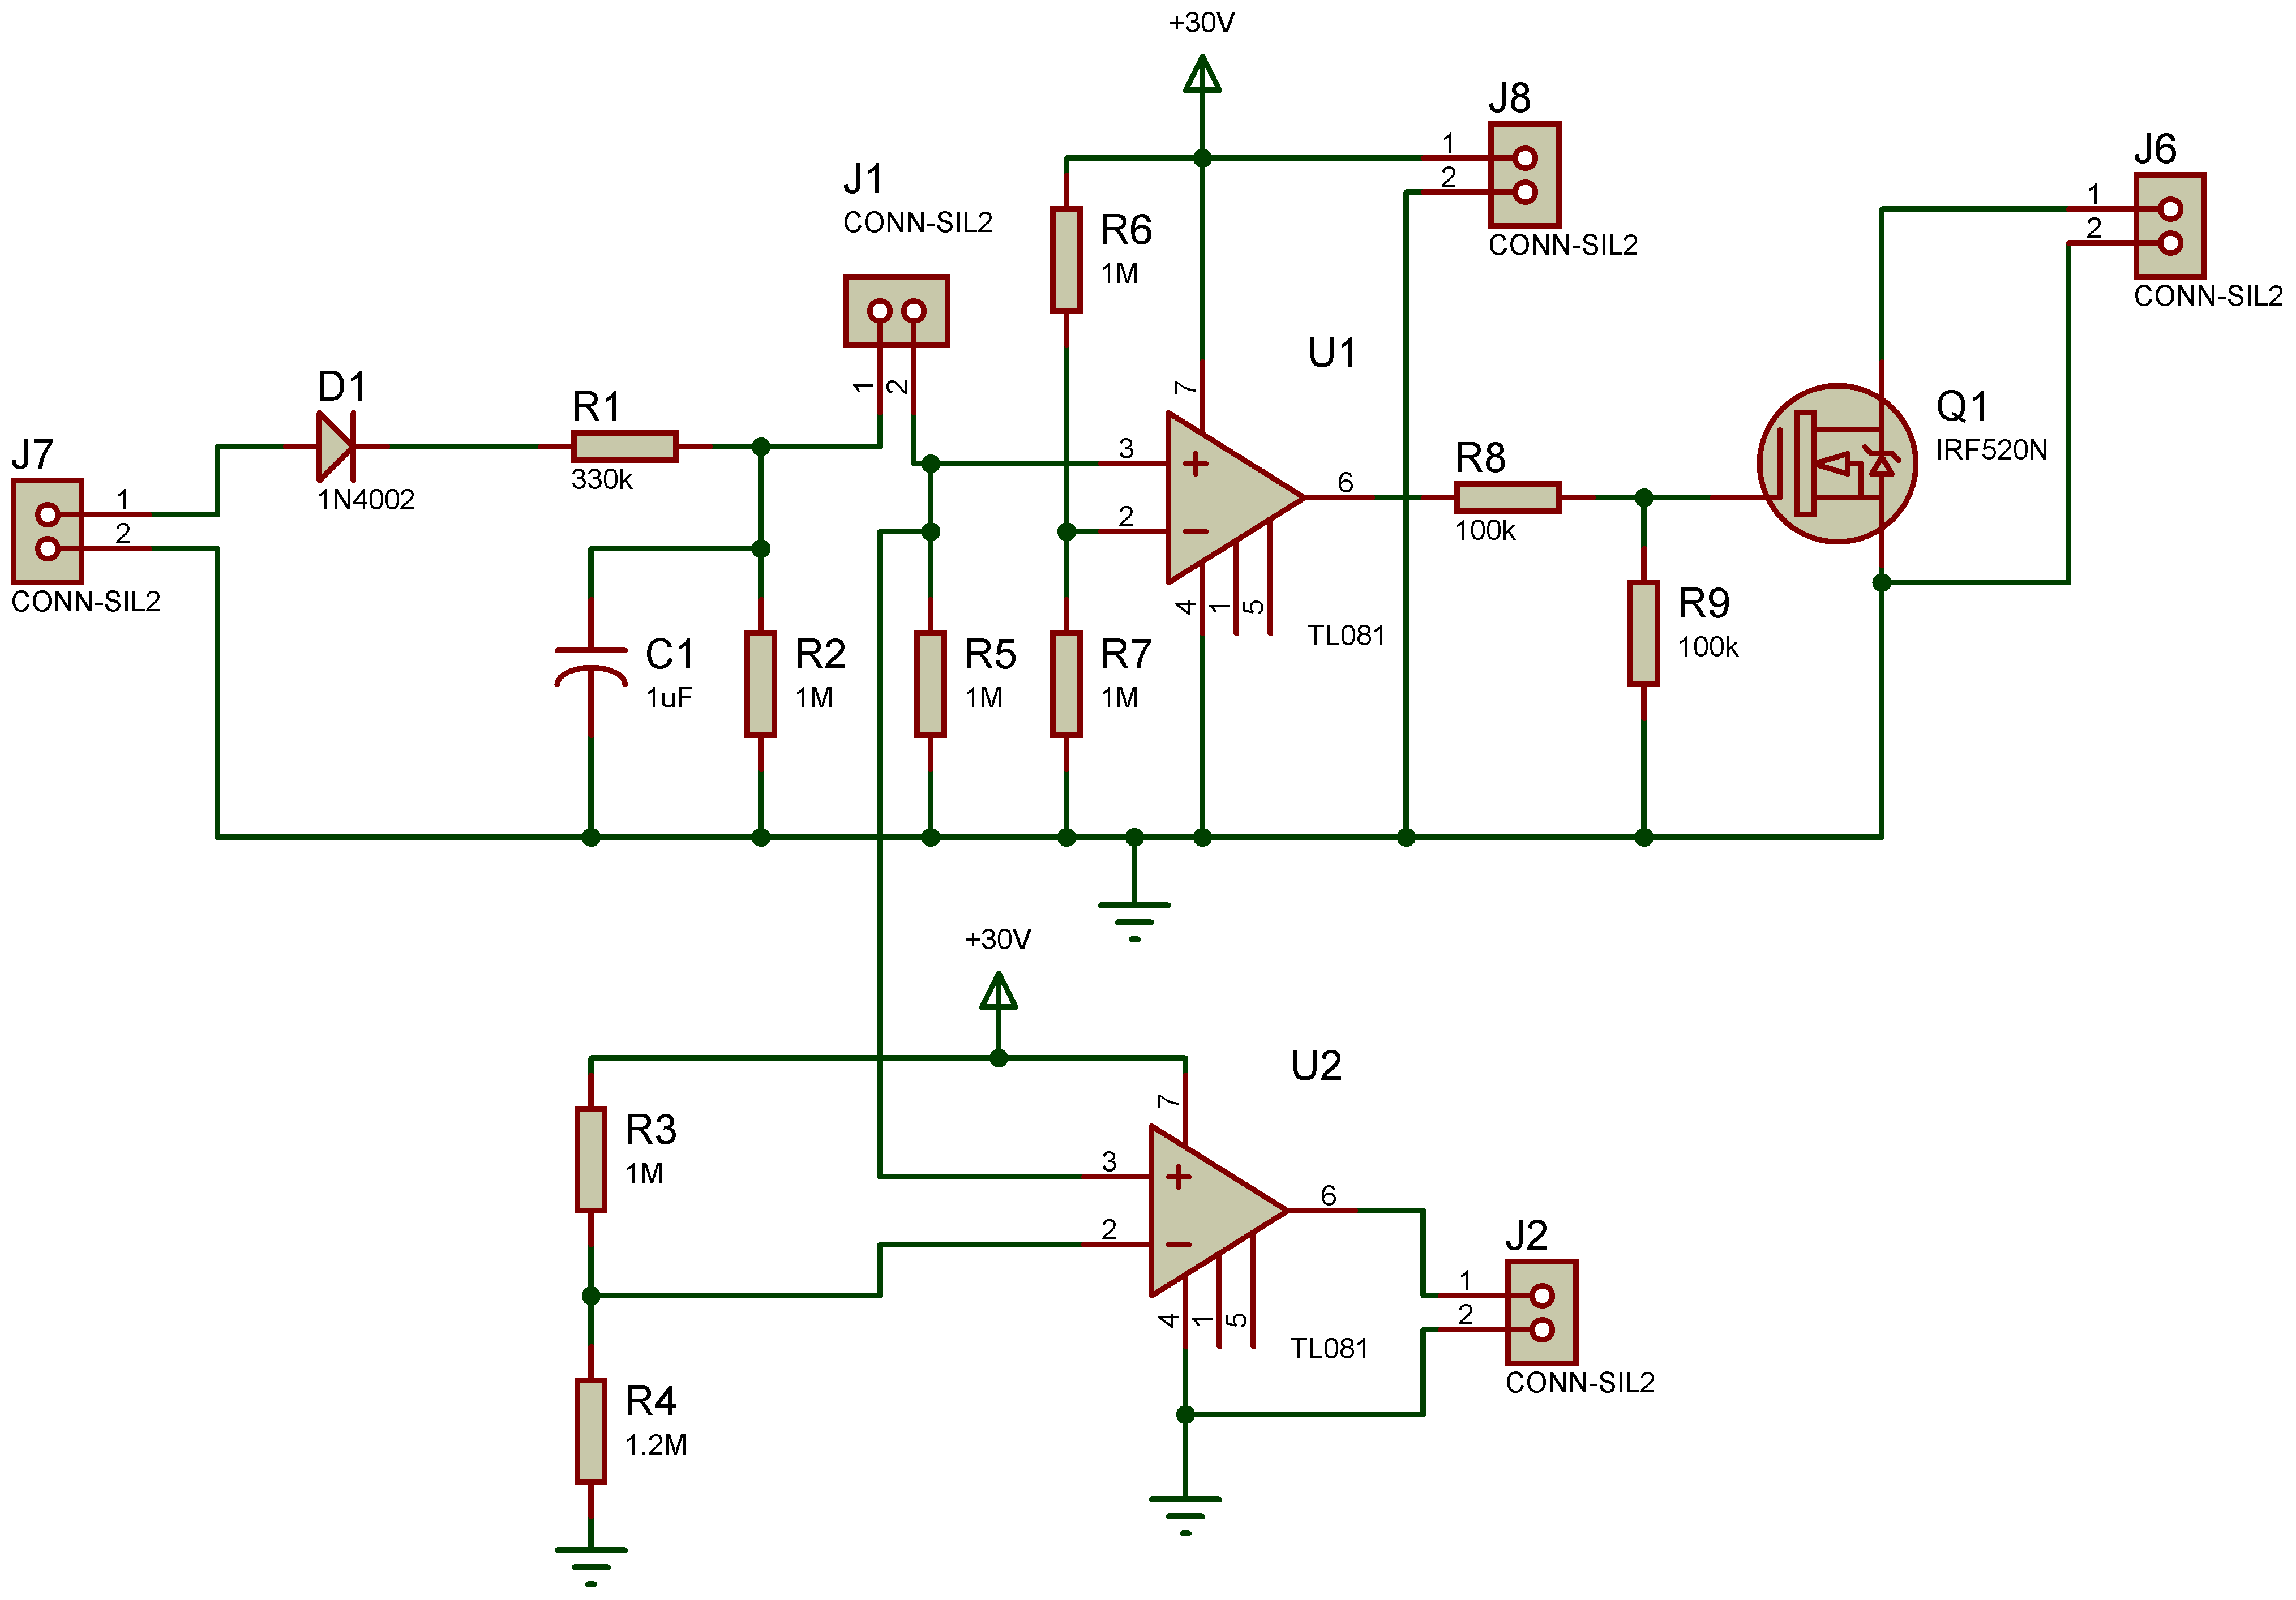
\includegraphics[width=0.99\textwidth]{../Proteus/Exports/Relaisansteuerung.png}
    \caption{Schaltplan der Platine zur Relaisansteuerung}
\end{figure}
\textbf{Anmerkung:}\\
Der OPV \textbf{U2} und die damit verbunde Klemme \textbf{J2} werden aufgrund einer nachträglichen Änderung im Schaltplan nicht mehr benötigt.
\newpage
\subsubsection{PCB-Layout}
\begin{figure}[h]
    \centering
    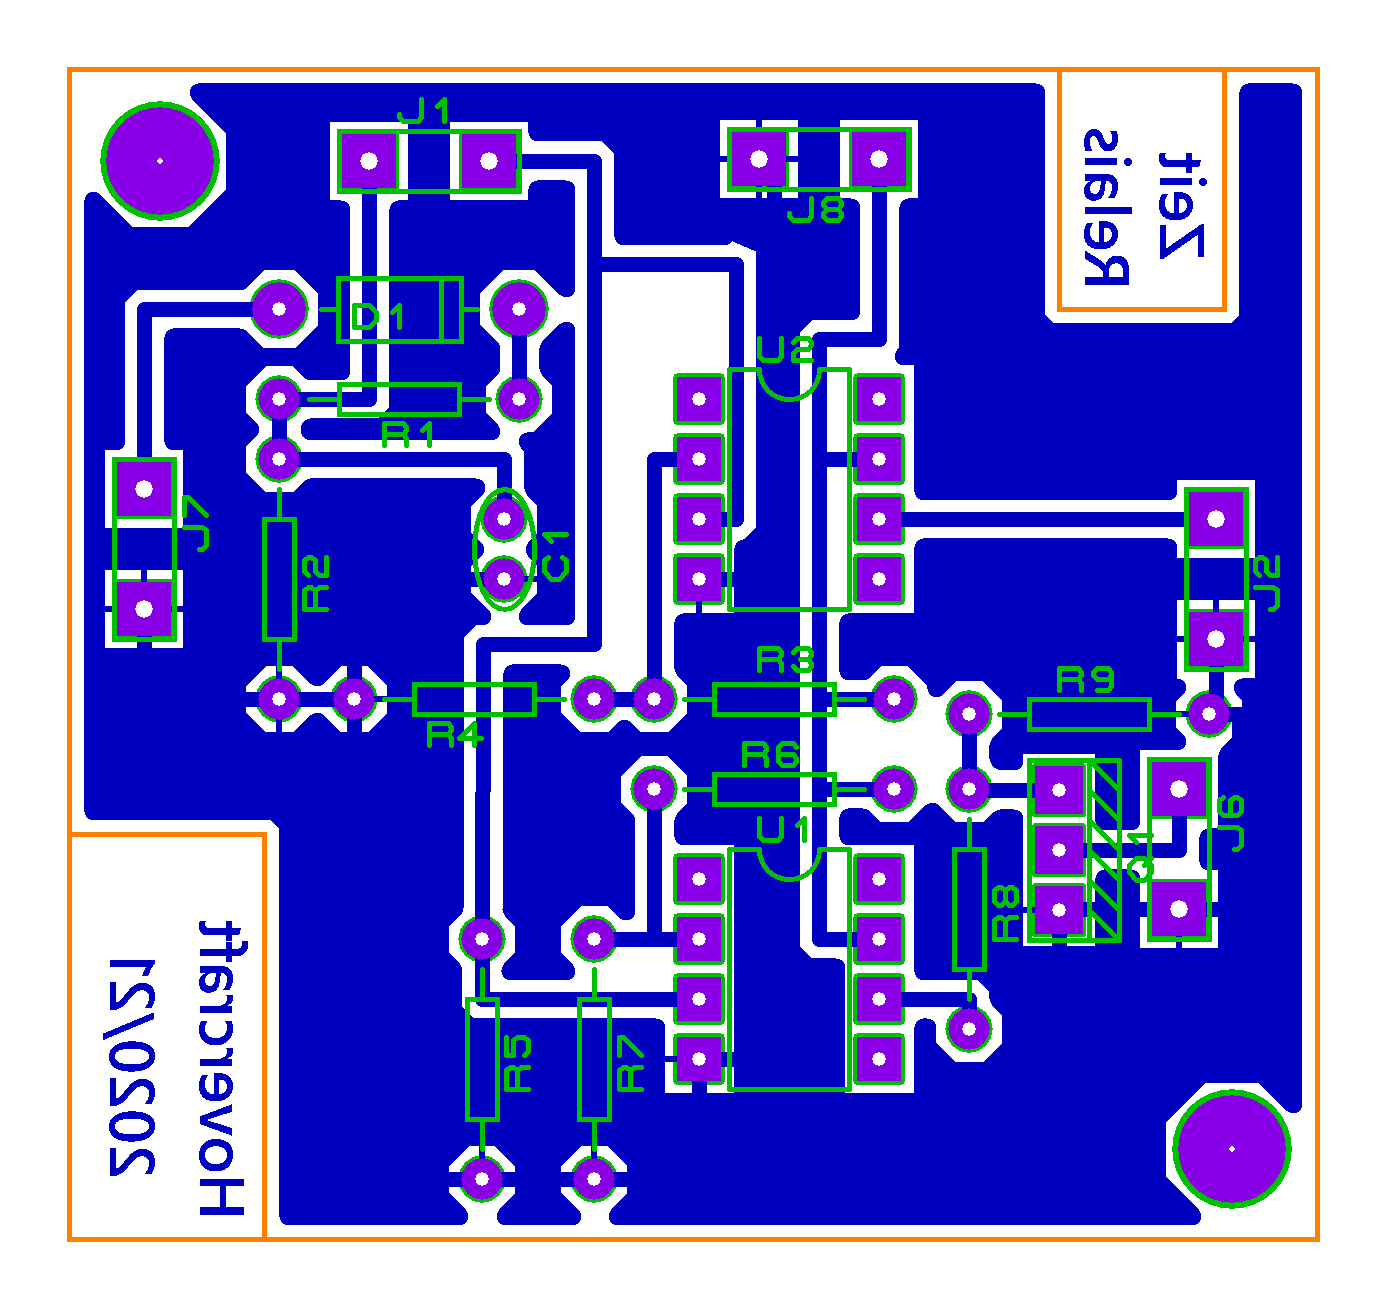
\includegraphics[width=0.95\textwidth]{../Proteus/Exports/Relaisansteuerung_PCB.png}
    \caption{PCB-Layout der Platine zur Relaisansteuerung}
\end{figure}
\newpage

\subsection{Platzierung am Boot}
Folgende \autoref{fig:Platinen:Aufbau_Rechts} \& \autoref{fig:Platinen:Aufbau_Links} zeigen die Position aller verbauten Platinen am Boot.

\begin{minipage}{\textwidth}
    \centering
    \begin{tikzpicture}
        \node[anchor=south west,inner sep=0] (image) at (0,0) {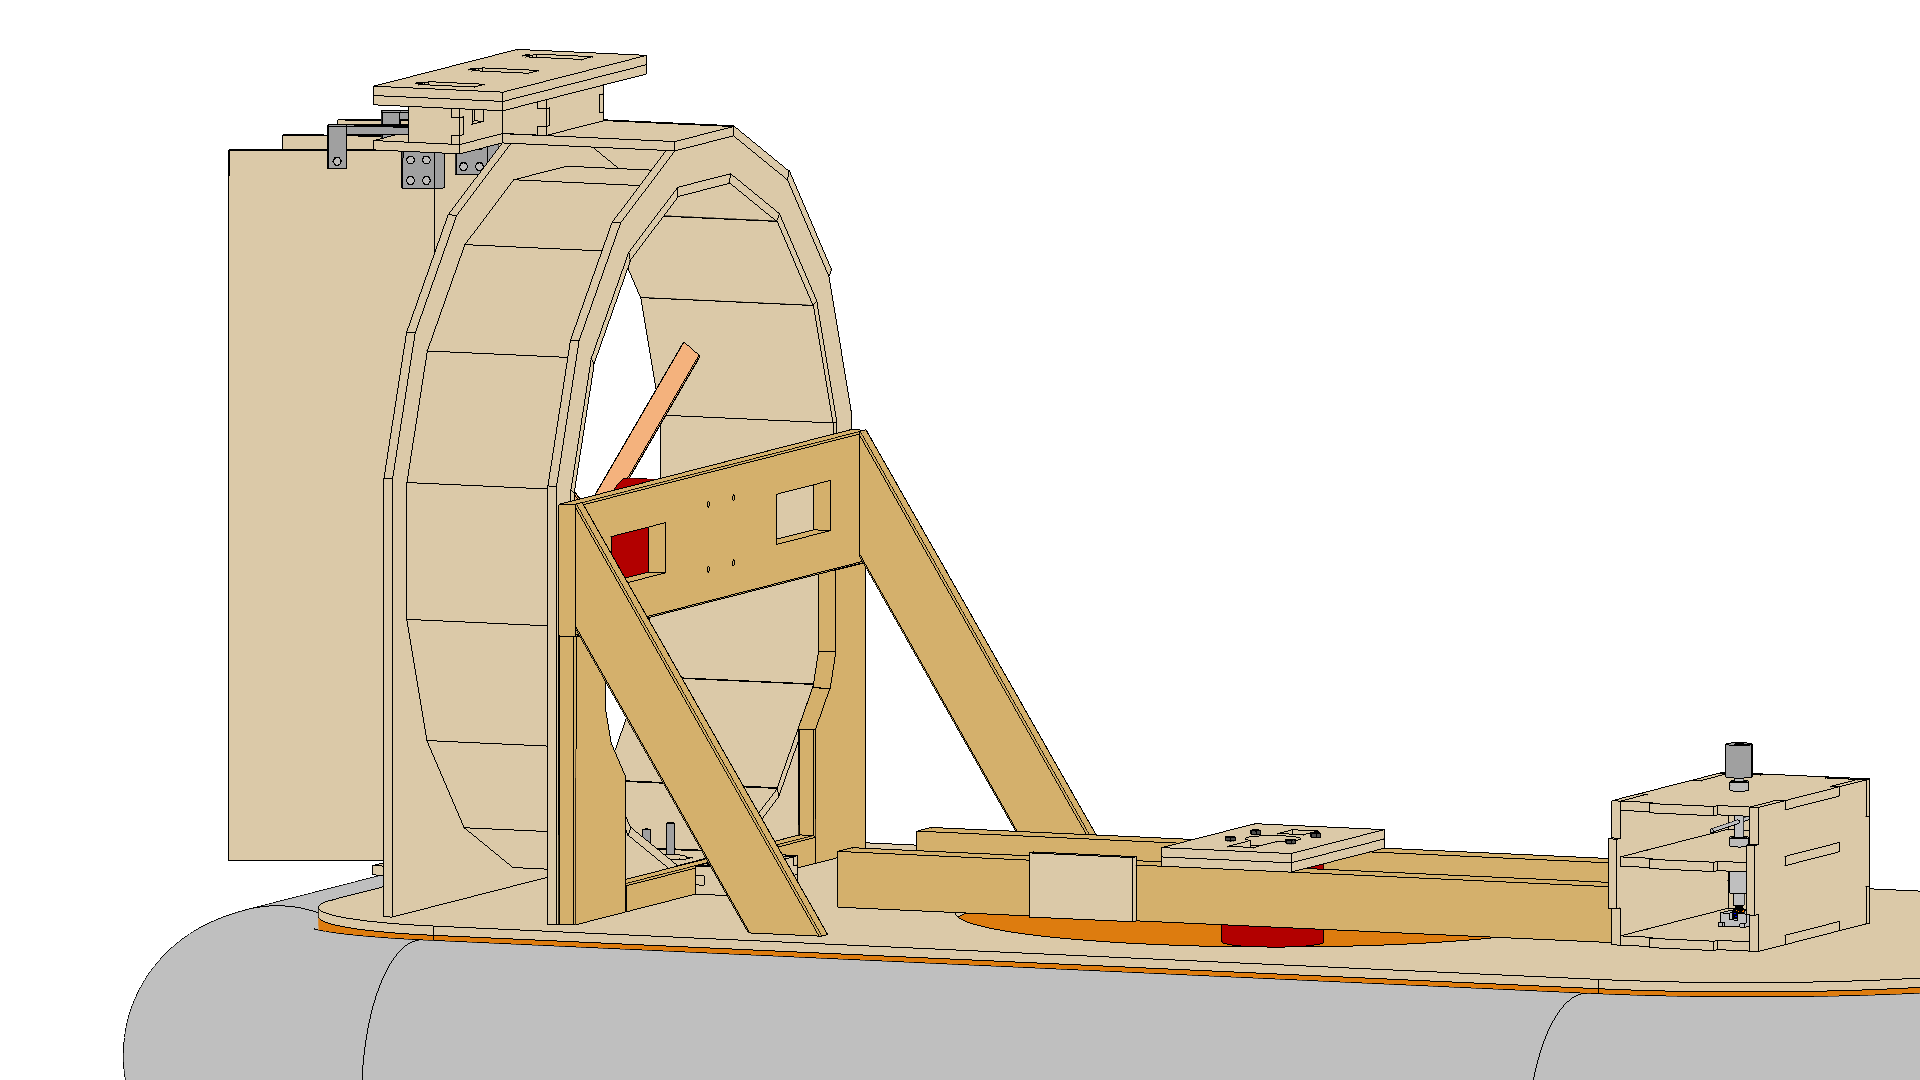
\includegraphics[width=0.85\textwidth]{../Inventor/PlatinenBilder/Seite1.png}};
        \begin{scope}[x={(image.south east)},y={(image.north west)}]
            \draw[blue,thick,->]  (0.66,0.85) -- (0.29,0.85) node [at start, above] {Temperatursensoren Rechts} -- (0.22,0.40);
            \draw[black,thick,->]  (0.66,0.75) -- (0.29,0.75) node [at start, above] {Relaisansteuerung} -- (0.27,0.60);
            \draw[red,thick,->]  (0.66,0.65) -- (0.29,0.65) node [at start, above] {Regler-hinten Platine}  -- (0.27,0.51);
            \draw[black,thick,->]  (0.66,0.55) -- (0.5,0.55) node [at start, above] {Regler-unten Platine} -- (0.47,0.19);
            \draw[Green,thick,->]  (0.54,0.45) -- (0.78,0.45) node [midway, above] {Lenker Platine} -- (0.89,0.14);
        \end{scope}
    \end{tikzpicture}
    \captionof{figure}{Platinen auf der rechten Seite des Bootes}
    \label{fig:Platinen:Aufbau_Rechts}
\end{minipage}

\begin{minipage}{\textwidth}
    \centering
    \begin{tikzpicture}
        \node[anchor=south west,inner sep=0] (image) at (0,0) {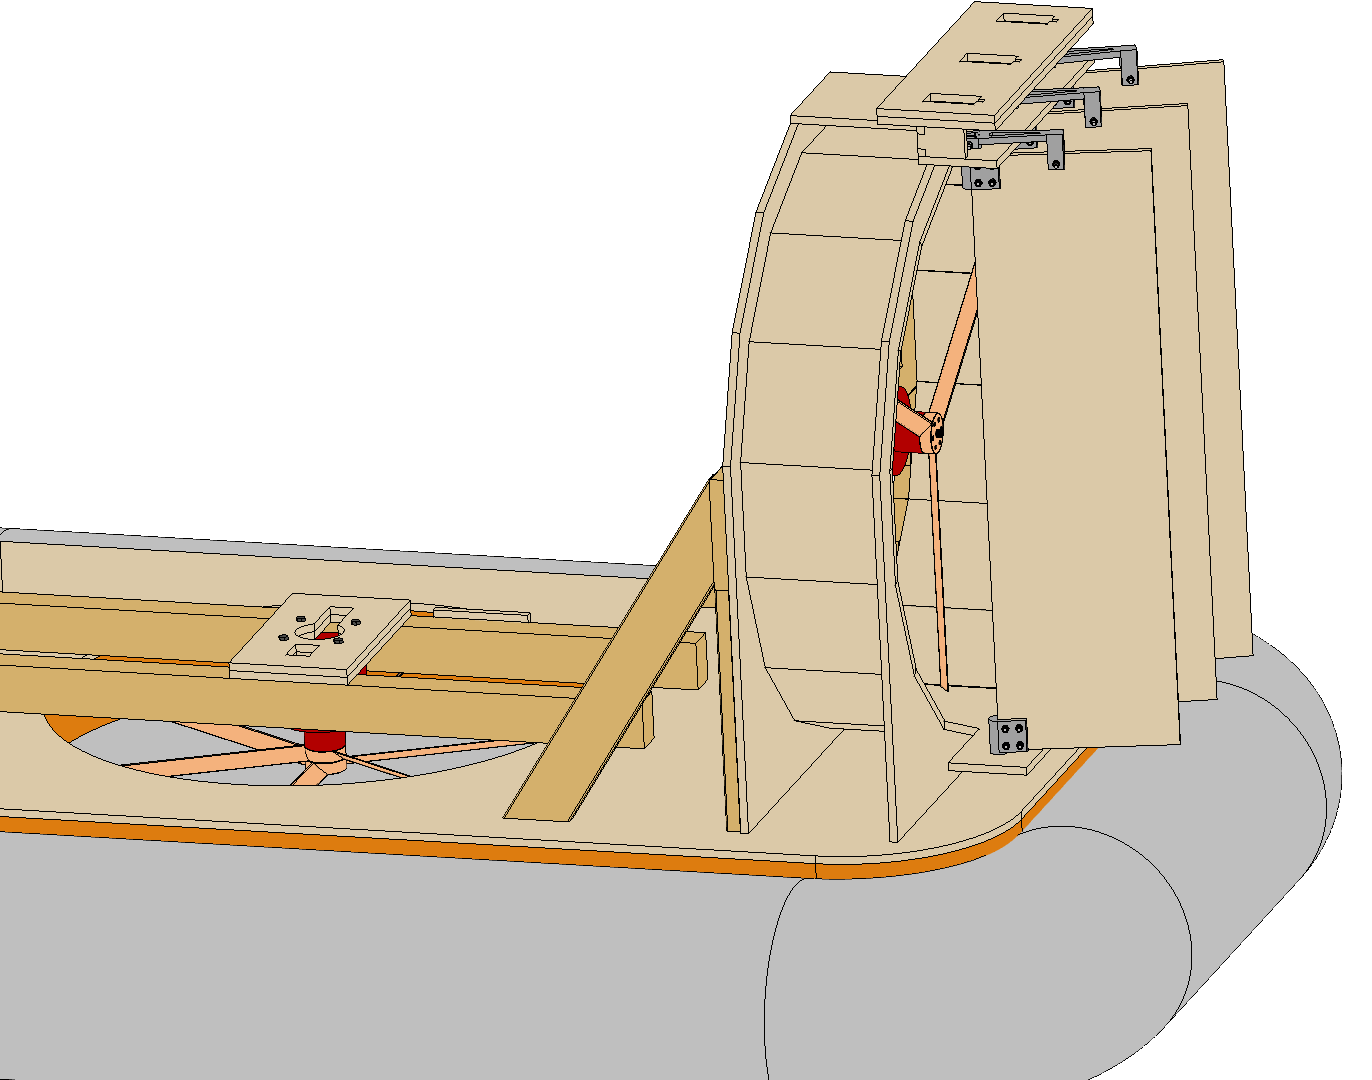
\includegraphics[width=0.85\textwidth]{../Inventor/PlatinenBilder/Seite2_2.png}};
        \begin{scope}[x={(image.south east)},y={(image.north west)}]
            \draw[red,thick,->]  (0.22,0.75) -- (0.5,0.75) node [midway, above] {Servo-ADC Platine}  -- (0.6,0.61);
            \draw[blue,thick,->]  (0.22,0.85) -- (0.5,0.85) node [midway, above] {Servo-Controller}  -- (0.61,0.81);
            \draw[black,thick,->]  (0.22,0.65) -- (0.49,0.65) node [near start, above] {Temperatursensoren Links}  -- (0.545,0.42);
        \end{scope}
    \end{tikzpicture}
    \captionof{figure}{Platinen auf der linken Seite des Bootes}
    \label{fig:Platinen:Aufbau_Links}
\end{minipage}

\newpage
